\renewcommand{\thechapter}{\arabic{chapter}}
\setcounter{chapter}{4}

\chapter{Diagnostic de l'image}
\label{chap:chapter_4}
\chapterintro
Comme évoqué durant le préambule, cette partie s'intéresse au premier niveau de diagnostic de notre processus global sur la modalité \gls{rcm}. Nous traiterons en d'autres termes, de la classification des images de cette modalité. Nous nous intéresserons à leur séparation selon trois annotations~: saine, bénigne ou maligne, mais également reviendrons à des considérations d'ordre médical de détection de malignité de ces images.\par

Ainsi, ce chapitre séparera plusieurs aspects dont dans un premier temps l'extraction de caractéristiques pertinentes par des méthodes manuelles mais également auto-déterminées à l'aide de réseaux profonds pré-entraînés, et dans un second temps la mise en œuvre de méthodes de classification éprouvées. Afin de rendre plus riche cette partie et de compléter nos conclusions, nous nous intéresserons également à l'influence de divers paramètres liés à la normalisation des caractéristiques, à la réduction de l'information dans le contexte de méthodes à fort nombre de dimensions, et à l'influence des données sur les résultats de classification.\par	
\newpage

%%%%%%%%%%%%%%%%%%%%%%%%%%%%%%%%%% 
%%%%%%%%%%%%%%%%% METHODOLOGIE
\section{Méthodologie}
La classification de la peau par méthode d'apprentissage est un problème très largement développé dans la littérature, notamment pour le mélanome. Néanmoins, dans le cadre plus particulier de la détection des \gls{lm} et \gls{lmm} sur base d'images \gls{rcm}, cette problématique n'a été abordé que par quelques articles~\cite{Halimi2017a, Halimi2017b, Wiltgen2008, Koller2011}. Nous nous intéresserons à la détection de cette pathologie au sein de la base d'image mise à disposition, et nous étudierons cette problématique selon divers angles d'approche~: 
\begin{inlinerate}
    \item d'une part la séparation des tissus malins, bénins et sains sous forme de problématique à 3 classes,
    \item et d'autre part, nous focaliserons sur la séparation entre les tissus malins et le reste des tissus sous forme de problématique binaire.
\end{inlinerate}\par

Afin de traiter ces problématiques, nous aborderons ces cas à l'aide de méthodes d'apprentissage supervisées, que nous déroulerons lors de ces prochains paragraphes. En effet, ces approches sont largement explorées dans des thématiques variées du domaine de l'imagerie médicale et également démontrées comme fonctionnelles~\cite{Litjens2017,Pathan2018}. Nous aborderons les prochains éléments selon un processus de classification classique, dans lequel nous adapterons certains des traitements en conséquence de notre problématique. Une vision macroscopique est présenté sur le schéma de la \Cref{fig:scheme_macro_image_classification}.\par

Le pré-traitement des images n'est pas considéré dans ce travail, car jugé peu utile sur des images \gls{rcm} et assez peu traité dans la littérature. Nous suivrons ce processus selon trois étapes majeures~:
\begin{inlinerate}
    \item l'extraction de caractéristiques,
    \item le pré-traitement avant classification,
    \item et les méthodes de classification.
\end{inlinerate}
Ainsi, nous consacrerons une sous-section pour chacun de ces points lors des prochaines sous-parties. Puis, nous présenterons la méthodologie propre au déroulement de ces expériences et critères d'évaluation, avant de procéder à l'analyse des résultats.\par

\begin{figure}[H]
\centering
    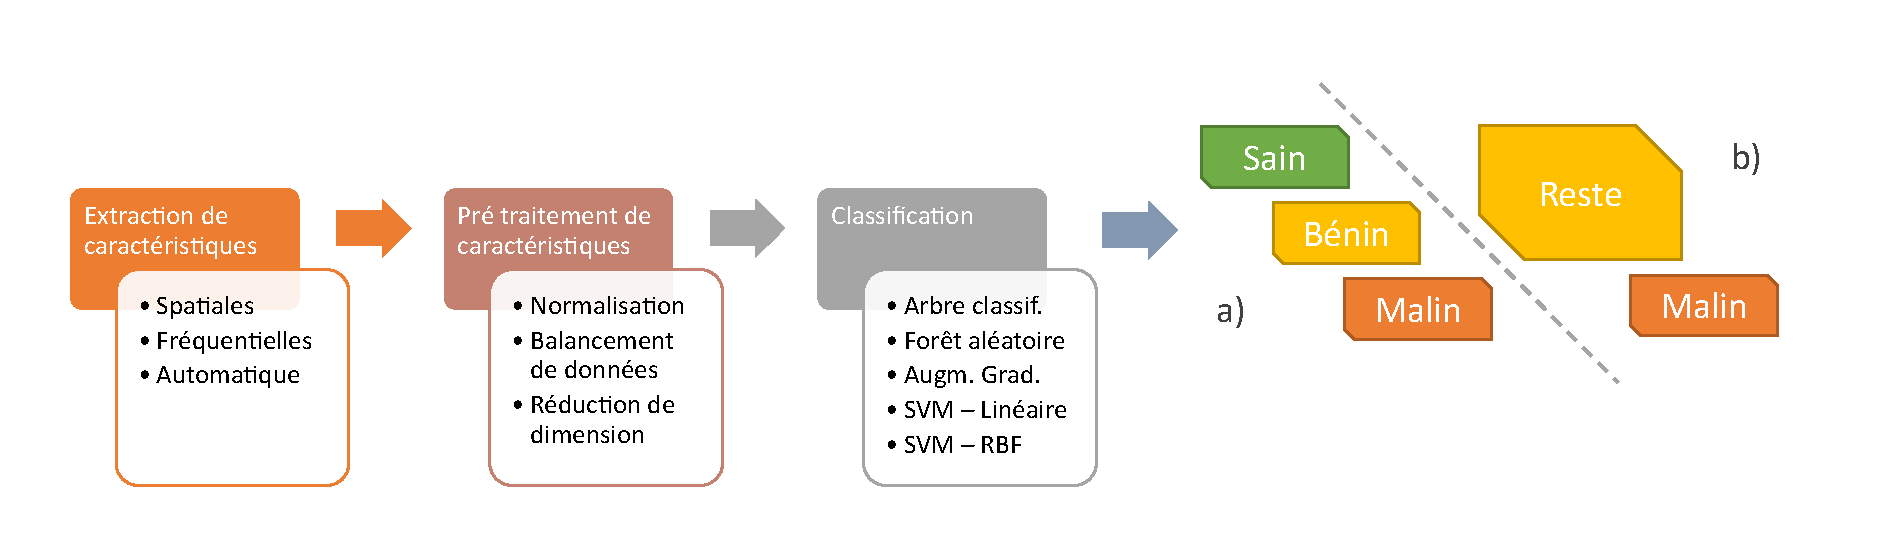
\includegraphics[width=\linewidth]{contents/chapter_4/resources/scheme_macro_image_classification.pdf}
    \caption{Représentation macroscopique du processus de diagnostic image suivi dans le cadre de l'apprentissage automatique. Nous arborerons une démarche la plus compréhensive, à 3 classes - a), mais également binaire par une emphase sur les images malignes - b).}
    \label{fig:scheme_macro_image_classification}
\end{figure}\par

\newpage

%%%%%%%%%%%%%%%%%%%%%%%%%%%%%%%%%% 
%%%%%%%%%%%%%%%%% FEATURES
\section{Méthodes d'extraction de caractéristiques}
\label{chap:feature_extraction}
L'étape d'extraction de caractéristiques consiste en l'obtention de valeurs dérivées à partir des données brutes dans le but de quantifier un phénomène. Ces valeurs jugées pertinentes sont ensuite utilisée pour la suite du traitement, généralement de la classification. Les éléments présentés en préambule visent à montrer l'importance des motifs de tissus, dont l'apparence varie selon~:
\begin{itemize}
    \item \textbf{la profondeur de l'acquisition} du tissus considéré, ainsi l'épiderme, \gls{dej} et le derme sont très différents du point de vue des tissus qui les constituent,
    \item \textbf{la pathologie à identifier}, les différentes lésions en notre possession sont assez différentes selon leur état bénin ou malin.
\end{itemize}
Les nombreux échanges menés auprès des dermatologues de notre étude clinique de référence ont également abouti à vérifier l'importance des aspects de textures au sein de leur processus cognitifs de décision vis-à-vis des pathologies de \gls{lm} et \gls{lmm}.\par

Nous traiterons des méthodes d'extraction de caractéristiques appliquées à nos images \gls{rcm}, que nous aborderons selon deux axes~:
\begin{inlinerate}
    \item d'une part les méthodes manuelles d'extraction de caractéristiques ou déterminées par un humain respectivement séparées en caractéristiques \textit{spatiales} et \textit{fréquentielles},
    \item d'autre part les méthodes non manuelles d'extraction de caractéristiques.
\end{inlinerate} 
L'appellation "manuelle" s'est ainsi imposée suite à l'apparition de réseaux de convolution profonds, afin de distinguer ces deux types d'approches~\cite{Nanni2017}.\par

\subsection{Méthodes manuelles d'extraction de caractéristiques spatiales}
L'extraction sur base d'information du domaine spatial est un champ de travail assez développé présentant comme avantage d'être intuitif mais pouvant être affecté par le bruit et autres phénomènes de dégradation de l'information. Ces opérations spatiales peuvent être décrites à deux niveaux d'interprétation, d'une part celui des valeurs brutes dont les descripteurs de premier ordre font partie mais ne fournissent aucune valeur de cohérence spatiale et, d'autre part celui par transformation de l'information initiale dont les descripteurs de second ordre ou plus font partie. Ces dernières méthodes prennent en compte la relation d'une valeur locale à celle de son voisinage~\cite{Kamila2015}.\par

Les descripteurs de premier ordre s'appliquent ainsi aux valeurs d'intensité ou à la distribution de celles-ci, sans traitement préalable. La \Cref{tab:first_order_descriptors} recense la plupart de ces caractéristiques issues de la distribution des valeurs brutes. Néanmoins, ces mesures tendent à ressortir des phénomènes globaux de l'image, mais ne suffisent pas à elles seules à analyser des motifs présents~\cite{Tomita1990, Srinivasan2008, Uyun2013, NyeinNyeinHlaing2015}. Ces mesures ont notamment été utilisées comme un complément de classification~\cite{Wiltgen2008}.\par

\begin{table}[H]
    \centering
    \begin{tabular}{ll}
        \toprule
        \textbf{Mesure}             & \textbf{Expression mathématique}                                                  \\ \hline
        Moyenne                     & $\overline{x} = \frac{1}{n}\sum_{i=1}^n x_i$                                      \\   
        Variance                    & $v = \frac{1}{n}\sum_{i=1}^n \left(x_i - \overline{x}\right)^2$                   \\ 
        Entropie                    & $e = -\sum_{i=1}^n {\mathrm{P}(x_i) \log_b \mathrm{P}(x_i)}$                      \\
        Kurtosis                    & $k=\frac{r \sum_{i=1}^{n}\left(x_{i}-\bar{x}\right)^{4}}{\left(\sum_{i=1}^{n}\left(x_{i}-\bar{x}\right)^{2}\right)^{2}}-3$\\
        Asymétrie                   & $a = \mathbb{E} \left[ \left( \frac{X - \mu}{\sigma} \right)^3 \right]$           \\  
        \bottomrule
    \end{tabular}
    \caption{Liste de différentes mesures obtenues à partir du premier ordre.}
    \label{tab:first_order_descriptors}
\end{table}\par

Les descripteurs de second ordre, ou plus, utilisent l'information locale et en déduisent une relation à leur voisinage par l'utilisation d'une transformation intermédiaire. Parmi ces transformations, les plus courantes d'entre elles sont~: 
\begin{inlinerate}
    \item \gls{glcm},
    \item \gls{glrlm},
    \item et \gls{glszm}.
\end{inlinerate} 
L'extraction sur la base d'information du second ordre a notamment été traitée en 1973 pour de la reconnaissance sur des images aériennes et satellitaires, par Robert Haralick~\cite{Haralick1973}. Ce travail est une extension des \gls{glcm}, dont le principe consiste en un recensement des combinaisons d'intensité présentes dans une image. Cette extraction nécessite une direction dans laquelle les combinaisons seront recherchées, en 2D ces directions sont aux nombres de quatre~:
\begin{inlinerate}
    \item horizontale,
    \item verticale,
    \item et les deux diagonales opposées.
\end{inlinerate}
Le principe de fonctionnement des \gls{glcm} est schématisé en \Cref{fig:scheme_principle_GLCM} pour une extraction selon la direction horizontale. Le travail~\cite{Haralick1973} a ainsi démontré la pertinence des \gls{glcm} dans la différenciation d'images texturées, en calculant selon les quatre directions évoqué précédemment, quatorze critères statistiques. Ces divers critères statistiques sont recensés sur la \Cref{tab:haralick_descriptors}, ainsi que leurs formules associées. Afin de réaliser ces diverses extractions de manière optimale, nous avons recours à la bibliothèque logicielle "Mahotas"~\cite{coelho2012}.\par
 
\begin{figure}[H]
    \centering
    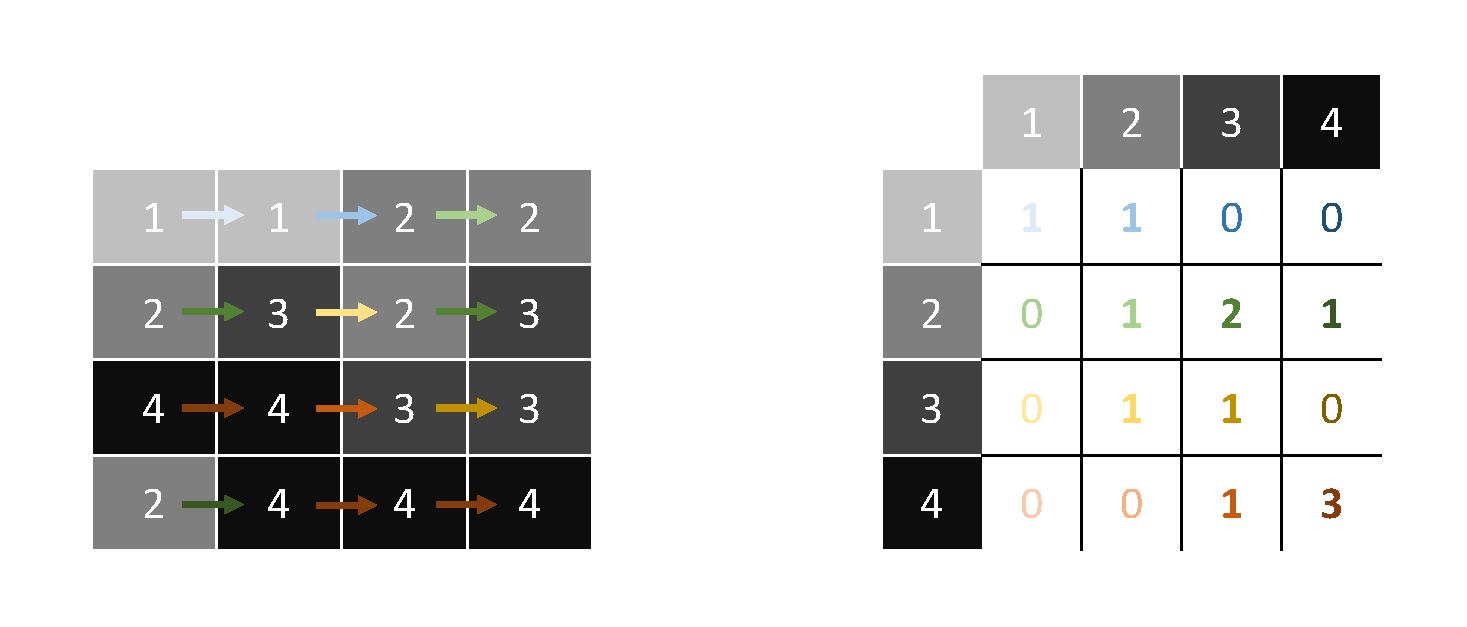
\includegraphics[width=\linewidth]{contents/chapter_4/resources/scheme_principle_GLCM.pdf}
    \caption{Représentation de la création d'une matrice sur base de \gls{glcm} selon la direction horizontale et dont la valeur de distance de voisinage est de 1. Les flèches représentent les diverses relations de voisinage horizontal, et leur couleur fait référence à leur emplacement dans la matrice de \gls{glcm}.}
    \label{fig:scheme_principle_GLCM}
\end{figure}\par

Les travaux menés par l'une des études sur les lésions mélanocytaire en \gls{rcm}~\cite{Wiltgen2008}, appuient ces deux catégories de mesures spatiales de l'information de texture. En effet, l'étude met en avant l'importance des douze premières caractéristiques formulées par Haralick~\cite{Haralick1973} et adjoint cinq mesures de premier ordre comme complément d'information dont~:
\begin{inlinerate}
    \item la moyenne,
    \item l'erreur quadratique moyenne,
    \item l'asymétrie de la répartition de l'histogramme,
    \item le kurtosis (mesure d'aplatissement de la distribution),
    \item et l'entropie.
\end{inlinerate}
Ce même travail met en avant que la texture des lésions de la peau ne possède pas d'orientation particulière. Afin de rendre ces caractéristiques plus robustes aux rotations et, de réduire la quantité d'informations extraite, ses auteurs préconisent l'utilisation d'une moyenne sur les quatre directions. Ainsi, cette manipulation permet de réduire l'information à unique vecteur de taille 1$\times$12 pour ces caractéristiques d'Haralick~\cite{Wiltgen2008}.\par

\begin{table}[H]
    \centering
    \begin{tabular}{ll}
        \toprule
        \textbf{Mesure}                     & \textbf{Expression mathématique}                                                              \\ \hline
        Moment Angulaire                    & $ \sum_i\sum_jp(i,j)^2$                                                                       \\
        Contraste                           & $\sum_{k=0}^{N_g-1} k^2 p_{x-y}(k)$                                                           \\
        Corrélation                         & $\frac{\Large{\sum_{i=1}^{N_g}\sum_{j=1}^{N_g}} (ij)p(i,j) - \mu_x\mu_y}{\sigma_x\sigma_y}$   \\
        Différence des Moments Inverse      & $\sum_{i=1}^{N_g}\sum_{j=1}^{N_g} \frac{1}{1 + (i - j)^2} p(i,j)$                             \\   
        Entropie                            & $-\sum_{i=1}^{N_g}\sum_{j=1}^{N_g} p(i,j) \log(p(i,j))$                                       \\   
        Somme - Moyenne                     & $\sum_{i=2}^{2N_g} i p_{x+y}(i)$                                                              \\    
        Somme - Variance                    & $\sum_{i=2}^{2N_g} (i - f_8)^2 p_{x+y}(i)$                                                    \\    
        Somme - Entropie                    & $\sum_{i=2}^{2N_g} (i - f_8)^2 p_{x+y}(i)$                                                    \\    
        Somme des carrés - Variance         & $\sum_{i=1}^{N_g}\sum_{j=1}^{N_g} (i - \mu)^2 p(i,j)$                                         \\   
        Différence - Variance               & ${\rm variance \ of ~} p_{x-y}$                                                               \\    
        Différence - Entropie               & $-\sum_{i=0}^{N_g-1} p_{x-y}(i) \log(p_{x-y}(i))$                                             \\
        Mesure de Corrélation 1             & $\frac{f_9 - HXY1}{\max(HX,HY)}$                                                              \\  
        Mesure de Corrélation 2             & $[1 - \exp(-2(HXY2 - f_9))]^{1/2}$                                                            \\ 
        Coefficient de Corrélation Maximal  & $(max(\sum_k \frac{p(i,k)p(j,k)}{p_x(i)p_y(k)}))^{1/2}$                                       \\ 
        \bottomrule
    \end{tabular}
    \caption{Liste des des différentes mesures proposée par Robert Haralick applicable aux \gls{glcm}.}
    \label{tab:haralick_descriptors}
\end{table}\par
 
Les expériences menées sur base de descripteurs manuels spatiaux se décomposeront en plusieurs temps. Tout d'abord, nous procéderons à une étude de l'importance séparée des mesures sur l'information de premier ordre et sur les mesures proposées par Haralick sur l'information de second ordre. Nous profiterons de l'expérience pour mesurer l'impact de la moyenne dans cette tâche. Puis, nous réemploierons la démarche de combinaison conjointe de ces mesures, menée par l'un des articles~\cite{Wiltgen2008}. Par ailleurs, la \Cref{tab:number_features_spatial} synthétise l'ensemble des méthodes d'extraction ainsi que le nombre associé de caractéristiques extraites.\par
\begin{table}[h]
    \centering
    \begin{tabular}{ll}
        \toprule
        \textbf{Méthode}                            & \textbf{Nombre de caractéristiques}   \\ \hline
        Mesures premier ordre                       & 14                                    \\ \hline
        Haralick~\cite{Haralick1973} - 4 directions & 56                                    \\ \hline
        Haralick~\cite{Haralick1973} - Moyenne      & 14                                    \\ \hline
        Wiltgen~\cite{Wiltgen2008} - Spatial        & 17 (12+5)                             \\
        \bottomrule                 
    \end{tabular}
    \caption{Liste des méthodes spatiales évaluées dans ce chapitre et leur nombre de caractéristiques extraites associées.}
    \label{tab:number_features_spatial}
\end{table}

\subsection{Méthodes manuelles d'extraction de caractéristiques fréquentielles}
L'extraction sur base d'information du domaine fréquentiel est également un champ de travail assez développé, notamment pour sa robustesse face aux perturbations telle que le bruit, ainsi que la vitesse d'exécution de certaines opérations telle que le filtrage. En revanche, l'information extraite est plus difficile d'interprétation et, nécessite une information spatiale suffisamment conséquente pour être juste~\cite{Kamila2015}. Ce dernier point est négligeable dans ce travail, nos données étant dotées d'une résolution spatiale suffisante de \SI{1000}{\px} $\times$ \SI{1000}{\px}.\par

Plusieurs courants majeurs de représentation fréquentielles sont utilisés, dont~: 
\begin{itemize}
    \item la Transformée de Fourier~\cite{Ursani2007, Smach2008a},
    \item la Transformée en cosinus discrète~\cite{Sorwar2001},
    \item la Transformée en ondelettes~\cite{Arivazhagan2003,Hong2010},
    \item et la Transformée de Gabor~\cite{Ursani2007}.
\end{itemize}
Notre travail se consacrera à deux de ces approches, d'une part à la transformée de Fourier et d'autre part à la transformée en ondelettes, toutes deux traitées sur des problématiques de classification similaires~\cite{Wiltgen2008,Halimi2017a,Halimi2017b}. Également, ces deux méthodes sont deux représentants majeurs des deux grandes familles de représentation en fréquences.\par

La transformée de Fourier se résume à la décomposition d'une donnée en une somme de fréquences. Dans le cas d'une image, cette transformation donne lieu à une représentation, dans laquelle~: les basses fréquences, au centre, représentent une forme d'homogénéité au sein d'une image ; tandis que les hautes fréquences, en extérieur, sont associées à de fortes zones de transitions. Cette transformation conserve également l'orientation des fréquences, représentés à l'aide d'un angle formé à partir de l'origine. En revanche, bien que la transformée de Fourier permette de décrire parfaitement la composition fréquentielle de l'image, elle ne peut en localiser la provenance des fréquences~\cite{Wiltgen2008}. Cet espace reste néanmoins approprié à la caractérisation d'images texturées, et a suscité un grand intérêt au milieu des années 1980~\cite{Persoon1986}. Différentes mesures ont été proposées dans cet espace afin de caractériser des textures~:
\begin{itemize}
    \item l'extraction d'information à partir \textbf{de cercles concentriques} réguliers~\cite{Smach2008a, Wiltgen2008} afin d'isoler l'information propre à chaque intervalle de fréquences (\Cref{fig:scheme_fourier_features} - a),
    \item l'extraction d'information à partir \textbf{de directions} en partance du centre vers l'extérieur de la transformée à angles constants ~\cite{Wiltgen2008} (\Cref{fig:scheme_fourier_features} - b).
\end{itemize}
Ces deux travaux préconisent l'extraction d'une valeur de moyenne et d'un écart-type sur différentes régions de l'espace fréquentiel afin de qualifier les phénomènes précédemment présentés~\cite{Smach2008a, Wiltgen2008}. 

L'une des expériences menée par Wiltgen~\cite{Wiltgen2008} se base sur la transformée de Fourier, et extrait \textbf{38 descripteurs} du spectre de magnitude~:
\begin{itemize}
    \item \textbf{22 descripteurs} correspondent à la moyenne calculée sur des rayons répartis de manière équidistante du centre du spectre (\Cref{fig:scheme_fourier_features} - a),
    \item \textbf{16 descripteurs} correspondent à la moyenne calculée sur des directions à intervalles constants (\Cref{fig:scheme_fourier_features} - b).
\end{itemize}
La transformée de Fourier sera effectuée dans le reste de ce travail par la bibliothèque logicielle "SciPy" \cite{Virtanen2020}.\par

\begin{figure}[h]
    \begin{center}
        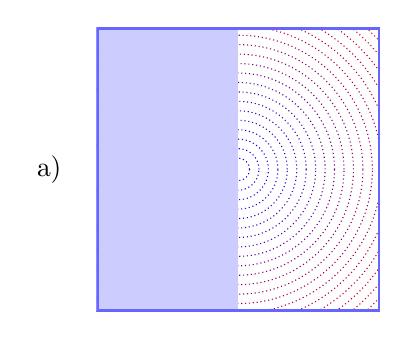
\begin{tikzpicture}[scale=1.2]
            \node[] at (-2, 0) {a)};
            \begin{scope}
                \clip (-1.5, -1.5) rectangle (1.5, 1.5);
                \foreach \cRadius in {1, ..., 22}
                    \pgfmathsetmacro\cColor{\cRadius/22*100}
                    \draw[red!\cColor!blue, densely dotted] (0, 0) circle (0.02+\cRadius*0.1); 
                    
                \fill[blue!20] (-1.5, -1.5) rectangle (0, 1.5);
                \draw[blue!60, ultra thick] (-1.5, -1.5) rectangle (1.5, 1.5);
            \end{scope}
        \end{tikzpicture}
        \qquad
        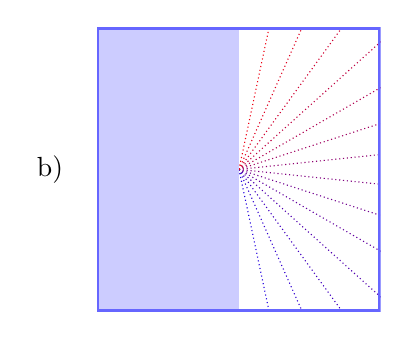
\begin{tikzpicture}[scale=1.2]
            \node[] at (-2, 0) {b)};
            \begin{scope}
                \clip (-1.5, -1.5) rectangle (1.5, 1.5);
                \foreach \cAngle in {1, ..., 16}
                    \pgfmathsetmacro\cColor{\cAngle/16*100}
                    \draw[red!\cColor!blue, densely dotted] (0, 0) -- (\cAngle* 180 / 15 -102:3); 
                \fill[blue!20] (-1.5, -1.5) rectangle (0, 1.5);
                \draw[blue!60, ultra thick] (-1.5, -1.5) rectangle (1.5, 1.5);
            \end{scope}
        \end{tikzpicture}
    \end{center}
    \caption{Schéma représentant l'extraction de caractéristiques à partir de l'espace de Fourier. En a), l'utilisation de cercles concentriques depuis l'origine, schématisé en pointillés ; En b), l'extraction selon une direction.}
    \label{fig:scheme_fourier_features}
\end{figure}\par

La transformée en ondelettes possède divers avantages dont une bonne capacité de localisation, par translation de l'ondelette mère, et la possibilité de prendre en considération plusieurs échelles d'analyse, par homothétie~\cite{Livens1997,Wiltgen2008}. Concernant le choix de l'ondelette mère, celui-ci ne semble pas affecter la qualité des caractéristiques extraites~\cite{Fatemi1996, Livens1997}. Néanmoins, l'un des auteurs préconise le choix d'ondelette symétrique ou anti-symétrique~\cite{Livens1997}. Plusieurs de nos références s'orientant vers des ondelettes de Daubechies ou de Haar, nous privilégierons ces dernières dans nos expériences~\cite{Wiltgen2008,Halimi2017a}. La décomposition en ondelettes sur images se réalise en 3 étapes successives~: 
\begin{inlinerate}
    \item de filtrage passe-bas et passe-haut horizontal,
    \item de filtrage passe-bas et passe-haut vertical,
    \item puis une étape de sous-échantillonnage afin de réduire la quantité d'informations généré apr ces deux précédentes étapes.
\end{inlinerate} Ce processus en trois temps est schématisé en \Cref{fig:scheme_dwt}. Nous effectuerons la transformée en ondelettes de ce travail à l'aide de la bibliothèque logicielle "PyWavelets"~\cite{lee2006}.\par

\begin{figure}[H]
    \centering
    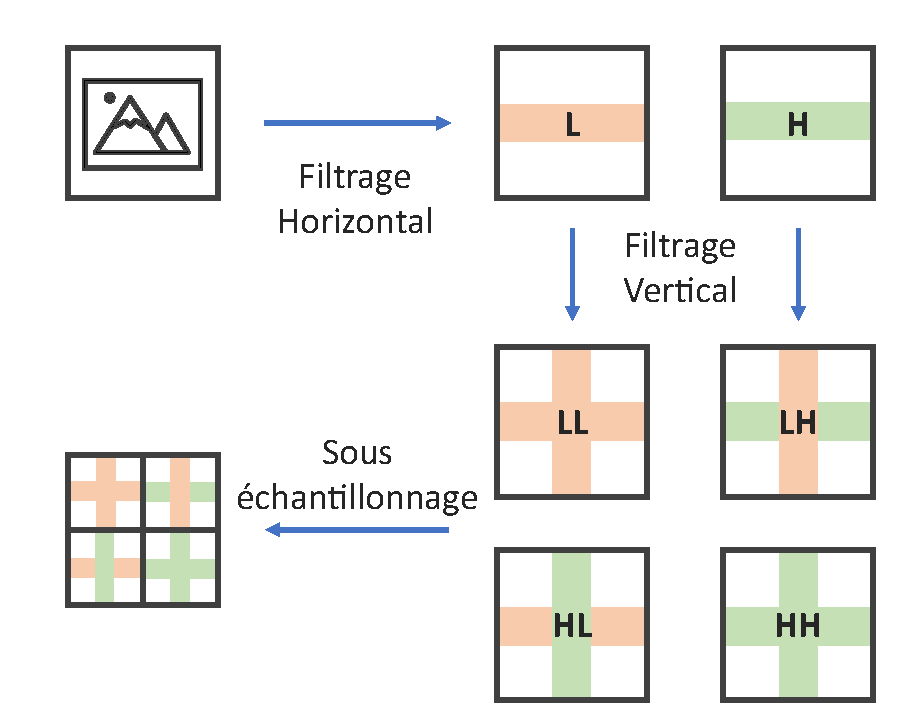
\includegraphics[width=0.7\textwidth]{contents/chapter_4/resources/scheme_dwt.pdf}
    \caption{Principe de la décomposition en ondelettes appliquée aux images~\cite{Livens1997}. La décomposition est réalisée en trois temps. Un filtrage passe bas (L) et passe haut (H) sont réalisés selon la direction horizontale, puis selon la direction verticale. Enfin, un sous échantillonnage de coefficient 2 est appliqué afin d'obtenir une matrice de même taille que l'image d'origine.}
    \label{fig:scheme_dwt}
\end{figure}\par 

Ainsi, nous réaliserons plusieurs de ces expériences sur base de descripteurs en fréquence. Dans un premier temps, nous tenterons d'étudier l'efficacité de la transformation de Fourier et de la transformation en ondelettes (à l'aide des ondelettes mère de Daubechies et de Haar) sur la séparation des classes. Puis dans un second temps, nous reproduirons la méthode de la littérature employant une combinaison de descripteurs de l'espace de Fourier~\cite{Wiltgen2008}. La \Cref{tab:number_features_frequency} synthétise le nombre associé de caractéristiques extraites par ces diverses méthodes d'extraction fréquentielles.\par

\begin{table}[H]
    \centering
    \begin{tabular}{ll}
        \toprule
        \textbf{Méthode}                        & \textbf{Nombre de caractéristiques}   \\ \hline
        Fourier                                 & 10 / 20 / 30                          \\ \hline
        Ondelettes de Daubechies                & 12                                    \\ \hline
        Ondelettes de Haar                      & 12                                    \\ \hline
        Wiltgen~\cite{Wiltgen2008} - Fourier    & 38 (22+16)                             \\
        \bottomrule
    \end{tabular}
    \caption{Liste des méthodes fréquentielles évaluées dans ce chapitre et leur nombre de caractéristiques extraites associées.}
    \label{tab:number_features_frequency}
\end{table}\par

\subsection{Technique d'apprentissage par transfert de connaissances}
Les techniques d'apprentissage par transfert de connaissances sont un champ d'application relativement récent des techniques d'apprentissage automatique. Le principe est de réutiliser des connaissances précédemment acquises, dans le but de résoudre de nouveaux problèmes plus rapidement voire plus efficacement. Pour cela, ce champs vise à proposer des techniques permettant la transposition de connaissance d'une ou plusieurs tâches sources à une tâche cible~\cite{QiangYang2010}.\par

Le phénomène conjoint d'engouement pour les \gls{cnn} et la complexité des architectures récentes pour le traitement des images a accentué les recherches en ce sens. En effet, les techniques d'apprentissage par transfert de connaissance sont une réponse efficace à de nombreuses problématiques autour de l'entraînement des \gls{cnn}, comme~: 
\begin{itemize}
    \item les \textbf{contraintes de suffisance de données}, notamment de données convenablement structurées et annotées disponible publiquement,
    \item le \textbf{complexité de l'entraînement}, comprenant le réglage des divers paramètres de ces réseaux (augmentations des données, fonction d'optimisation, \ldots),
    \item et les \textbf{contraintes matérielles nécessaires}, regroupant les aspects matériels dédiés au support de l'entraînement de ces architectures.
\end{itemize}\par

Certains domaines d'application ont vu apparaître de nombreuses bases de données publique, contribuant à résoudre partiellement la contrainte liée aux données. Ces bases ont également pour objectif de permettre de mesurer les performances de système de traitement de l'image, nous retrouvons notamment~: 
\begin{inlinerate}
    \item la \textbf{base MNIST}, pour mesurer l'aptitude de systèmes dédiés à la reconnaissance de chiffres manuscrit~\cite{lecun2010},
    \item les \textbf{bases CIFAR10 et CIFAR100}, permettant l'évaluation de systèmes de reconnaissance d'objets sur des image miniatures~\cite{Krizhevsky}, 
    \item et plus récemment, la \textbf{base ImageNet} pour la reconnaissance d'objets sur des images de taille commune~\cite{Deng2008}. 
\end{inlinerate}\par

Actuellement, la base ImageNet est l'une des plus sollicités pour entraîner et évaluer les architectures de \gls{cnn} actuelles. Outre leurs tailles, cette base propose des niveaux d'annotations variées, dont 1000 classes sont proposées. De plus, une très grande diversité d'échantillons est mise à disposition pour chaque classe pour un total de plus de 14 millions d'images. Selon certaines études, ce nombre d'images reste néanmoins sur-dimensionné vis-à-vis du nombre d'éléments nécessaires à l'entraînement de ces réseaux~\cite{Huh2016}.\par

Parallèlement à ce phénomène de mise à disposition de bases de données, sont ouverts publiquement des défis visant à démontrer l'efficacité de chaînes de traitement pour gérer ces données. De nombreuses avancées ont été réalisées sur la base ImageNet, à l'aide d'architectures de \gls{cnn} régulièrement dévoilés et mise à disposition de la communauté. Parmi ces réseaux nous pouvons citer les réseaux AlexNet~\cite{Krizhevsky2012}, GoogLeNet~\cite{Szegedy2015}, VGG~\cite{Simonyan2014}, Inception-V3~\cite{Szegedy2016}, ResNet~\cite{He2016} et Inception-ResNet~\cite{Szegedy2017}, avec respectivement comme précisions 0,54, 0,68, 0,71, 0,76, 0,78, and 0,80 sur la base ImageNet~\cite{Canziani2016}.\par

Néanmoins, la mise à disposition de la communauté de ces bases de données massives et de ces architectures ne permettent pas de lever les deux verrous liées au contraintes d'entraînement et matérielles de ces réseaux. C'est donc particulièrement le partage de modèles de \gls{cnn} pré-entraînés, couplé aux principes d'apprentissage par transfert de connaissances, qui ont suscités l'intérêt de nombreux travaux dont certains appliqués à de l'imagerie médicale~\cite{Litjens2017}. Ainsi, la majeure partie de ces réseaux pré-entraînés sont obtenus à l'aide de la base ImageNet, bien qu'aucune justification formelle n'ait été fournie à ce propos~\cite{Huh2016}.\par
 
\begin{figure}[H]
    \centering
    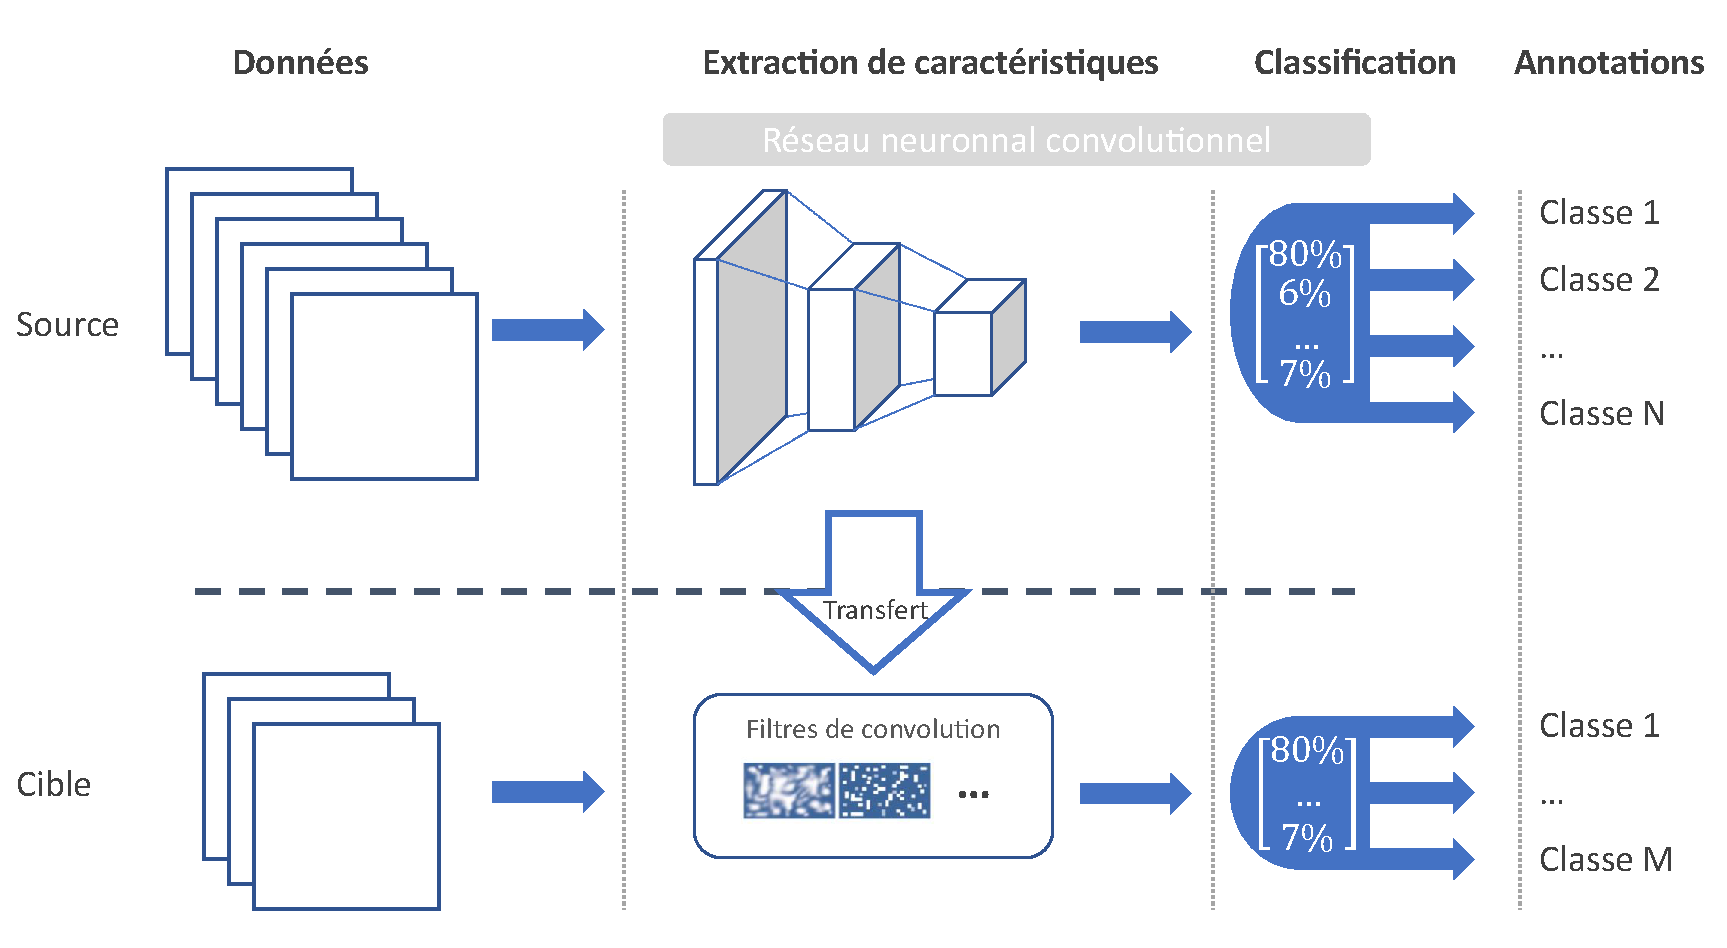
\includegraphics[width=\linewidth]{contents/chapter_4/resources/scheme_transfer_learning.pdf}
    \caption{Schéma représentant l'apprentissage par transfert par \gls{cnn}. Le réseau est entraîné sur des données et annotations d'une problématique \textit{source}. Puis, les paramètres de la partie liée à l'extraction de caractéristiques sont conservés et réemployés au sein d'une nouvelle problématique \textit{cible}.}
    \label{fig:scheme_transfer_learning}
\end{figure}\par

L'apprentissage par transfert sur \gls{cnn} se décompose en deux procédés majeurs~: 
\begin{inlinerate}
    \item d'une part l'extraction de caractéristiques moins coûteuse en ressources matérielles et temps,
    \item et d'autre part le réglage fin qui nécessite à l'inverse plus de temps et de ressources matérielles. 
\end{inlinerate}
Au sein de cette partie, nous nous focaliserons sur l'extraction de caractéristiques, schématisé en \Cref{fig:scheme_transfer_learning}, afin de limiter les contraintes d'apprentissage. Le principe consiste dans un premier temps à retirer les couches responsables de la classification du problème cible, puisque spécifiques au problème initial. Ces couches sont généralement des couches dites totalement connectées, qui vont pondérer l'importance des zones d'activation jusqu'au classes respectives. Dans un second temps, les couches responsables de l'extraction de caractéristiques sont conservées puis figées, en partant du postulat que ces caractéristiques sont suffisamment variées et adaptées à d'autres problématiques du traitement d'image. Enfin, ces couches sont combinées à de nouvelles couches totalement connectées ou à des modèles de classification~\cite{Litjens2017}.\par 

A cette fin, une première stratégie consiste à aplatir l'information des couches d'extraction par une étape de "Flatten" (littéralement "Applatissement"), transformant celle-ci d'un format de matrice 3D à un vecteur 1D (voir \Cref{fig:scheme_global_pooling} - Gauche). Néanmoins, l'une des problématiques résultantes concerne la dimension spatiale souvent importante de ces caractéristiques extraites. En effet, la dimension spatiale de ces données sera réduite par les couches convolutionelles selon leurs paramètres dépendants de l'architecture choisie. Ainsi, les paramètres de décalage, de pas ou encore de taille du noyau de convolution sont autant de paramètres qui affecterons la dimension spatiale de sortie. Pour pallier à cette information conséquente, des couches dites de "Global pooling" ont été introduites dans la littérature, et consistent à réduire l'information spatiale d'une carte d'activation à une unique valeur (voir \Cref{fig:scheme_global_pooling} - Droite). Les principales fonctions mises à disposition sont la fonction maximum et moyenne, donnant respectivement lieu à des couches de "Global Maximum Pooling" et "Global Average Pooling". D'autres fonctions sont également développées, mais la littérature s'accordera à préférer l'utilisation des couches de "Global Maximum Pooling"~\cite{christlein2019}.\par

\begin{figure}[H]
    \centering
    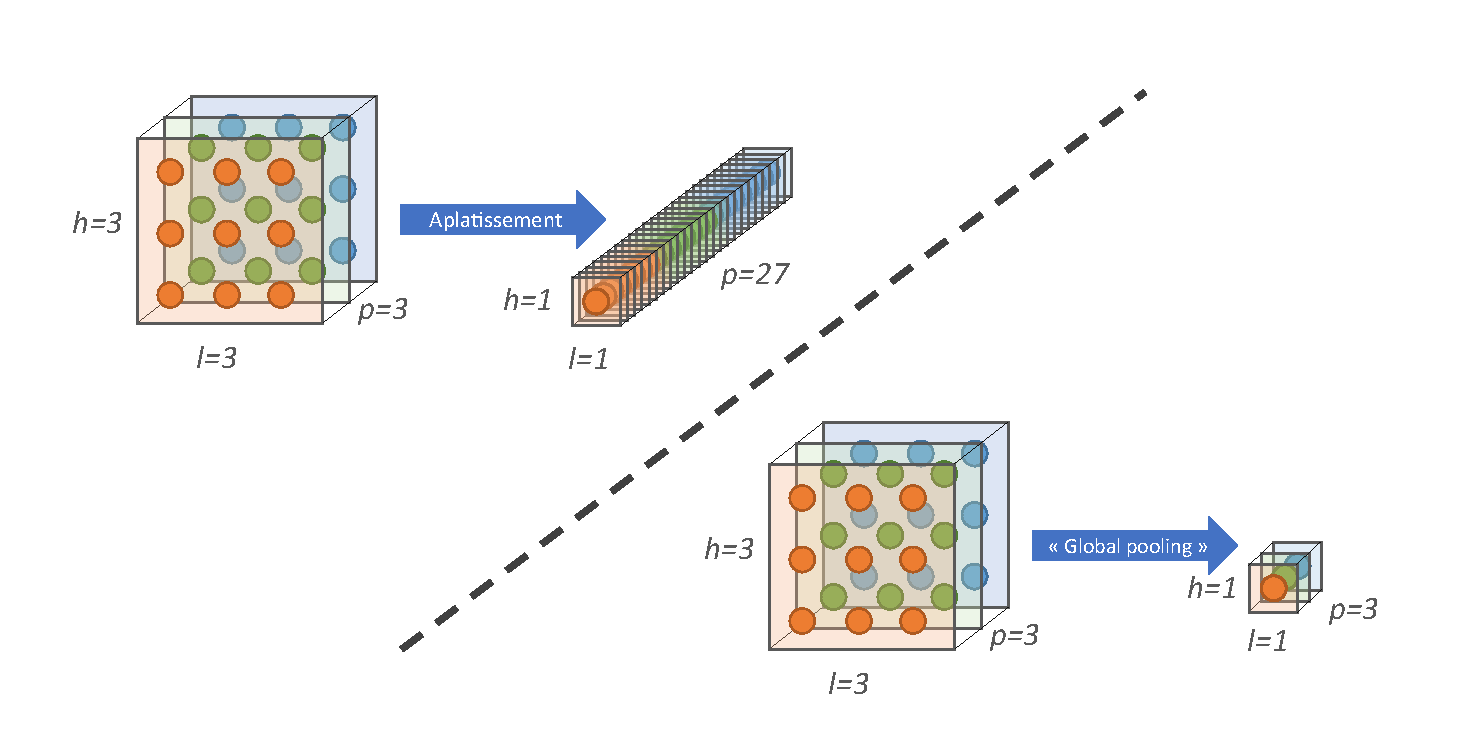
\includegraphics[width=\linewidth]{contents/chapter_4/resources/scheme_global_pooling.pdf}
    \caption{Schéma représentant l'aplatissement et la réduction d'information par "Global Pooling" au sein de \gls{cnn}. Le réseau est entraîné sur des données sources, généralement plus complètes. Puis, les paramètres de la partie liée à l'extraction de caractéristiques sont conservés et réemployé au sein d'une nouvelle problématique cible.}
    \label{fig:scheme_global_pooling}
\end{figure}\par

Bien que la plupart des travaux en imagerie médicale s'oriente vers l'architecture Inception-V3, son efficacité n'a pas été formellement démontrée au sein des applications médicales. La principale raison la plus probable expliquant le choix de cette architecture est la mise à disposition de ses modèles pré-entraînés par la plupart des librairies de \gls{cnn}~\cite{Litjens2017}. Les différentes expériences que nous mènerons sur l'apprentissage par transfert se focaliseront sur des architectures relativement récentes pré-entraînées sur la base d'image ImageNet et proposées par la bibliothèque "Keras Applications"~\cite{chollet2015a}. Afin de traiter les images dans leur intégralité, nous ne nous baserons que sur des réseaux dont les couches d'extraction de caractéristiques sont purement convolutionnelles et donc indépendantes de la taille de l'entrée. Ainsi, nous ne conserverons que quelques architectures de \gls{cnn} représentatives des avancés dans le domaine durant la dernière décennie, dont VGG, Inception-V3, ResNet et Inception-ResNet. L'ensemble des réseaux employés et nombre de paramètres extraits associés sont résumés au sein de la \Cref{tab:number_features_transferlearning}. Finalement, la manipulation des \ac{cnn} est réalisée à haut niveau grâce à la bibliothèque logicielle "Keras"~\cite{chollet2015} et sera couplée à la bibliothèque de bas niveau "Tensorflow"~\cite{tensorflow2015}.\par

\begin{table}[H]
    \centering
    \begin{tabular}{lll}
    \toprule
    \textbf{Architecture}               & Global Pooling   & \textbf{Nombre}    \\ \hline
    \multirow{2}{*}{VGG-16}             & Maximum          & 512                \\ \cline{2-3}
                                        & Moyenne          & 512                \\ \hline
    \multirow{2}{*}{Inception-V3}       & Maximum          & 2048               \\ \cline{2-3}
                                        & Moyenne          & 2048               \\ \hline
    \multirow{2}{*}{ResNet}             & Maximum          & 2048               \\ \cline{2-3}
                                        & Moyenne          & 2048               \\ \hline
    \multirow{2}{*}{Inception-ResNet}   & Maximum          & 1536               \\ \cline{2-3}
                                        & Moyenne          & 1536               \\
    \bottomrule
    \end{tabular}
    \caption{Liste des architecture de \gls{cnn} employés dans ce chapitre et leur nombre de caractéristiques extraites associées.}
    \label{tab:number_features_transferlearning}
\end{table}\par

\subsection{Analyse préliminaire des méthodes d'extraction}
Cette analyse préliminaire de l'information a pour but de montrer l'impact des méthodes d'extraction de caractéristiques précédemment citées sur le jeu de données en notre possession. Nous nous pencherons d'une part sur l'observation de deux images typiques de tissus malin et bénin par l'application des transformations et d'autre part, nous étudierons la capacité de séparation de chacune des méthodes précédentes sur l'ensemble des images.\par

Tout d'abord, il est intéressant de constater en général, la présence de motif plus lisses et moins contrastés au sein des images bénignes que des images malignes. L'application de \gls{glcm} de premier ordre sur nos images typiques est visible sur la \Cref{fig:example_glcm}. Il est possible d'observer une uniformité de cette information quelle que soit la direction observée, allant dans le sens de l'utilisation de la moyenne sur les caractéristiques proposées par Haralick~\cite{Wiltgen2008}. Enfin, cette transformation montre une certaine cohérence des transitions dans les images avec des valeurs présentes en majorité sur la diagonale. Néanmoins, ce phénomène semble plus intense sur l'image bénigne, traduisant des transitions plus douces que sur l'image maligne.\par

\begin{figure}[H]
    \centering
    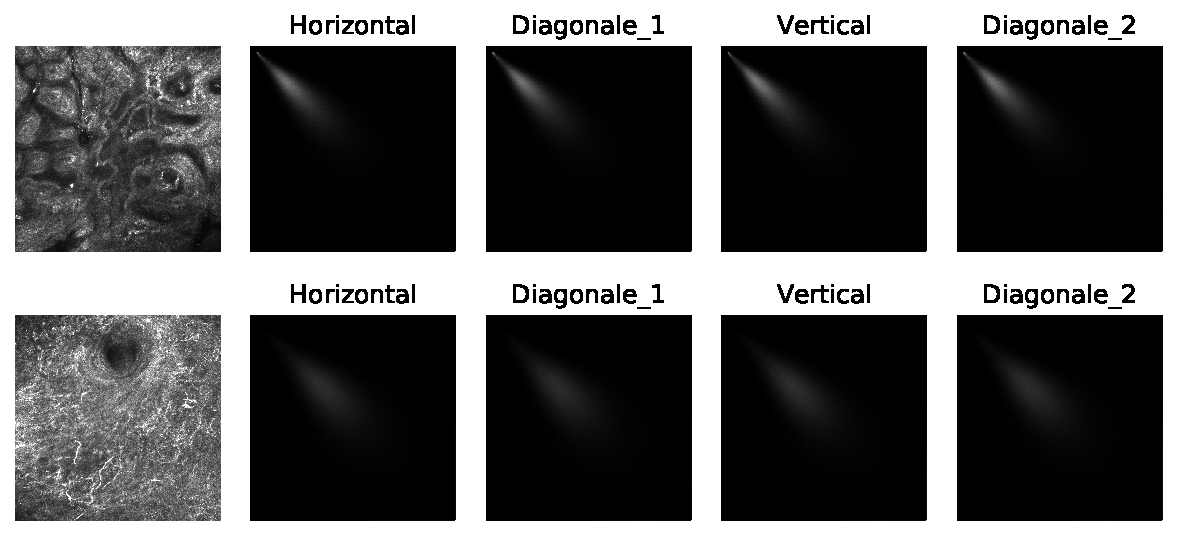
\includegraphics[width=\linewidth]{contents/chapter_4/resources/example_glcm.pdf}
    \caption{Exemple d'extraction de \gls{glcm} de second ordre sur deux images typique. En haut, un cas d'image bénigne ; En bas, une image pathologique typique de \gls{lm}.}
    \label{fig:example_glcm}
\end{figure}\par

La \Cref{fig:example_fft} met en application la transformée de Fourier centrée sur ces deux même images. L'observation du module de cette transformation permet de constater une information plus présente en intensité sur les basses fréquences que sur les hautes fréquences de l'image bénigne, là où sur l'image maligne cette information au centre forme une tâche plus diffuse. En revanche, à premier abord, la direction ne semble pas apporter d'information pertinente comme suggéré par l'article de Wiltgen~\cite{Wiltgen2008}.\par

\begin{figure}[H]
    \centering
    \includegraphics[width=\linewidth]{contents/chapter_4/resources/example_fft.pdf}
    \caption{Exemple de transformée de Fourier centrée appliquée à deux images typiques, représentation selon le module et la phase. En haut, un cas d'image bénigne ; En bas, une image pathologique typique de \gls{lm}.}
    \label{fig:example_fft}
\end{figure}\par

Enfin, nous terminons l'étude de ces deux exemples par l'application de décomposition en ondelettes. La \Cref{fig:example_wavelet_db4} reflète cette décomposition d'ondelettes de Daubechies tandis que la \Cref{fig:example_wavelet_haar} nous donne un aperçu de cette même méthode par ondelettes de Haar. Nous pouvons constater que les ondelettes de Haar semblent plus propices à isoler les zones de fortes transition que celle de Daubechies. Néanmoins, pour ces deux types d'ondelettes, les décompositions de l'image bénigne semble plus homogènes que celle de l'image maligne. De même, l'extraction des hautes fréquences sur l'axe vertical et horizontal semble plus adaptée que l'extraction combiné de ces deux axes pour l'image maligne.\par

\begin{figure}[H]
    \centering
    \includegraphics[width=\linewidth]{contents/chapter_4/resources/example_wavelet_db4.pdf}
    \caption{Exemple de transformée en ondelettes (Daubechies) appliquée à deux images typiques, à 2, 3 puis 4 niveaux. En haut, un cas d'image bénigne ; En bas, une image pathologique typique de \gls{lm}.}
    \label{fig:example_wavelet_db4}
\end{figure}\par

\begin{figure}[H]
    \centering
    \includegraphics[width=\linewidth]{contents/chapter_4/resources/example_wavelet_haar.pdf}
    \caption{Exemple de transformée en ondelettes (Haar) appliquée à deux images typiques, à 2, 3 puis 4 niveaux. En haut, un cas d'image bénigne ; En bas, une image pathologique typique de \gls{lm}.}
    \label{fig:example_wavelet_haar}
\end{figure}\par

Dans le but d'évaluer la séparation des classes, nous nous aiderons de l'\gls{pca}. En effet, malgré l'extraction de caractéristiques les données en notre possession contiennent un grand nombre de dimensions, rendant le problème difficile à analyser visuellement. De nombreuses techniques de réduction de l'information permettant une meilleure visualisation sont proposées dans la littérature, comme par exemple le T-SNE~\cite{Maaten2008} mais dont le principal inconvénient réside dans le nombre de degrés de liberté proposés. Néanmoins, l'\gls{pca} est une technique communément acceptée à cette fin~\cite{Himberg2001} et possède l'avantage de ne pas être dépendante de ce type de paramètres. Nous faisons également figurer la variance propre à ces deux axes, et pour chaque classe leur centre et leur dispersion sur la base de l'écart type.\par

Ainsi, la \Cref{fig:visualisation_spatial} met en évidence cette technique pour l'ensemble des méthodes d'extraction spatiales. Le premier constat concernant la variance expliquée est que ces deux axes semblent à même de fournir l'intégralité de la variance. Les données extraites à l'aide des techniques d'extraction de premier ordre ne semblent pas optimaux comme nous pouvons le constater sur \Cref{fig:visualisation_spatial}. En effet, les centres de masses et leur dispersion semble assez similaire, notamment pour les données bénignes et malignes. De plus, la séparation des classes ne semble pas marquée dans ces divers schémas d'extraction, et les classes de données vont jusqu'à se chevaucher pour les classes bénignes et saines pour les méthodes employant les caractéristiques d'Haralick. Par ailleurs, la distribution des méthodes employant ces caractéristiques d'Haralick semble similaire, suscitant de faibles différences entre elles.\par

\begin{figure}[H]
    \centering
    \begin{subfigure}{.45\textwidth}
      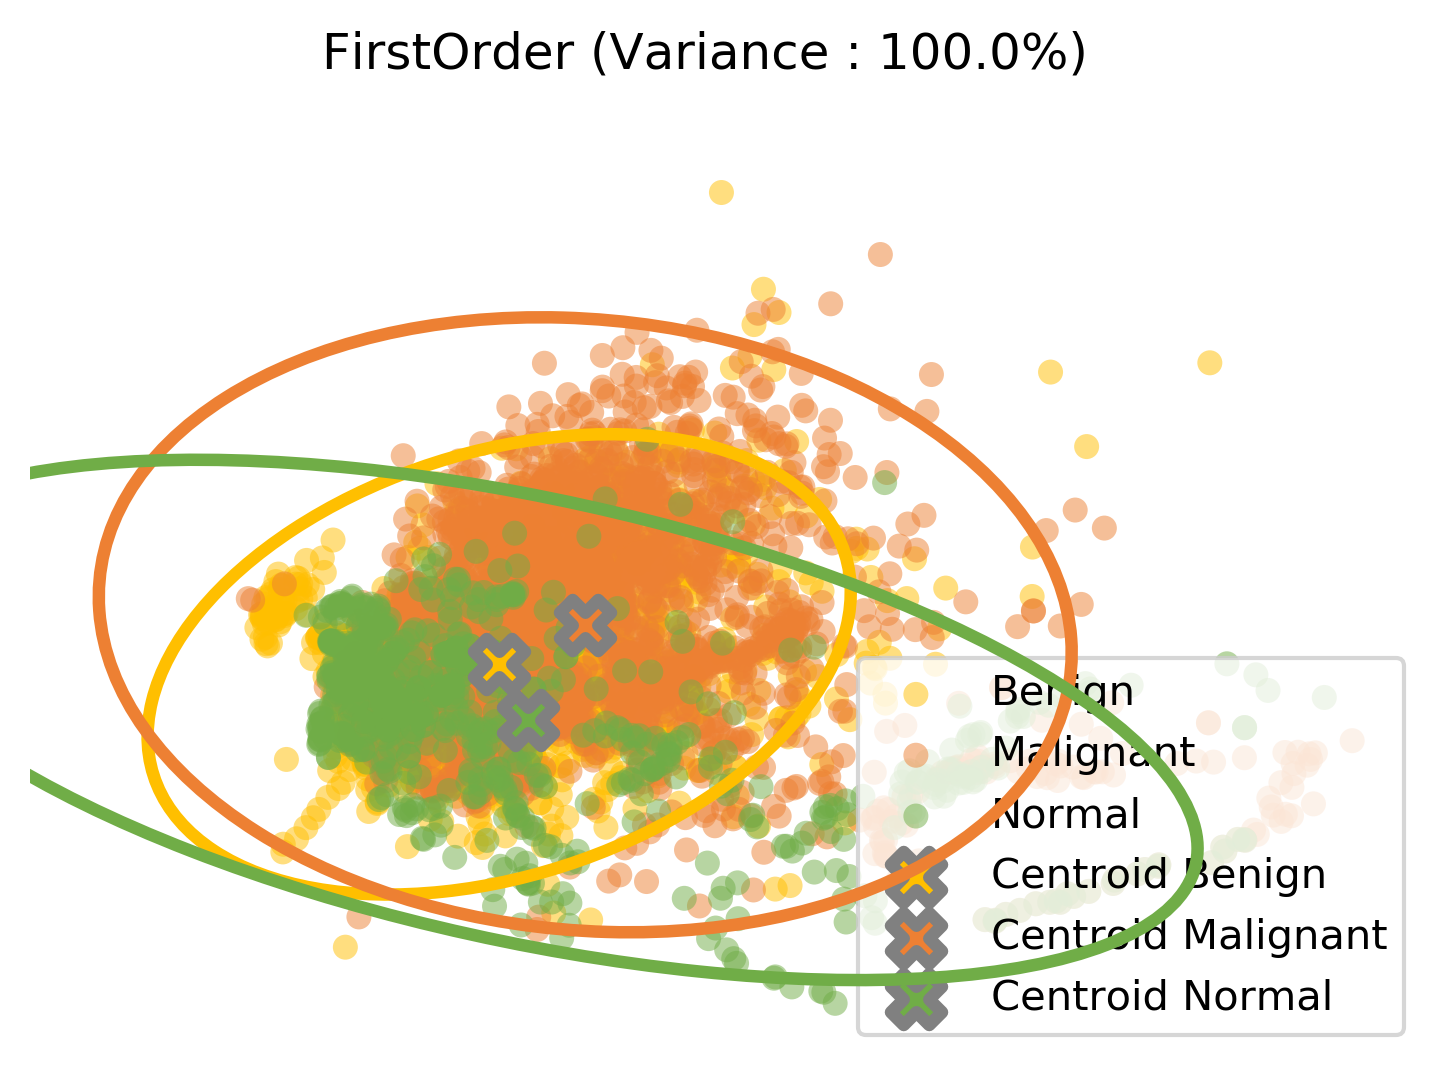
\includegraphics[width=\textwidth]{contents/chapter_4/resources/visualisation_spatial_FirstOrder.png}
    \end{subfigure}
    \begin{subfigure}{.45\textwidth}
      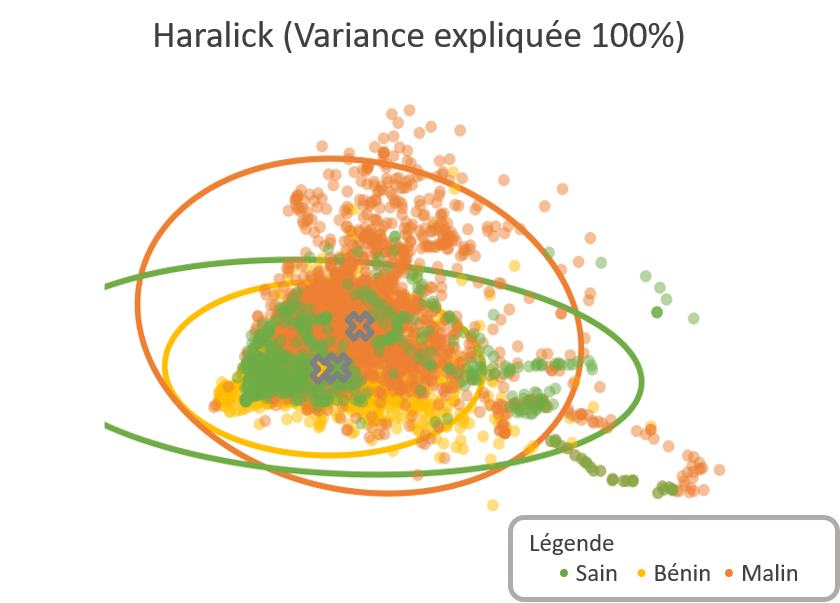
\includegraphics[width=\textwidth]{contents/chapter_4/resources/visualisation_spatial_Haralick.png}
    \end{subfigure}
    
    \begin{subfigure}{.45\textwidth}
      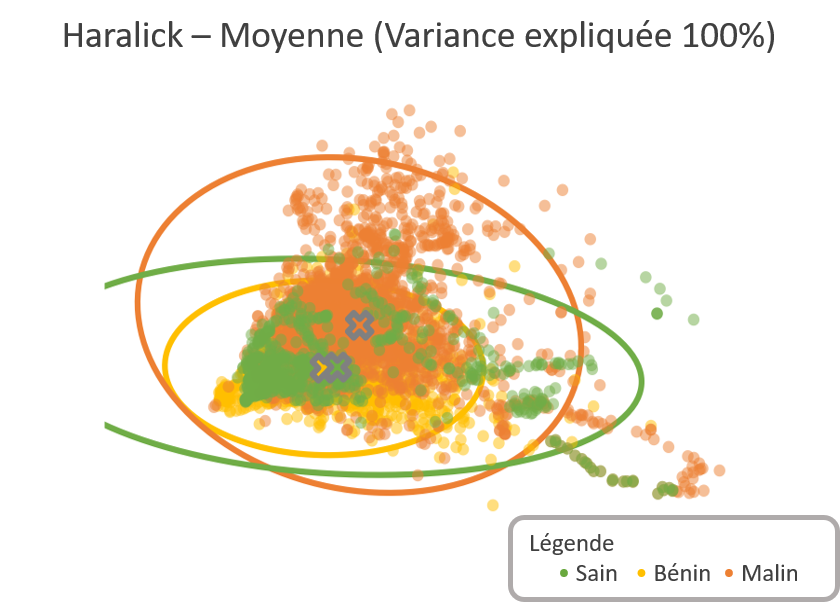
\includegraphics[width=\textwidth]{contents/chapter_4/resources/visualisation_spatial_HaralickMean.png}
    \end{subfigure}
    \begin{subfigure}{.45\textwidth}
      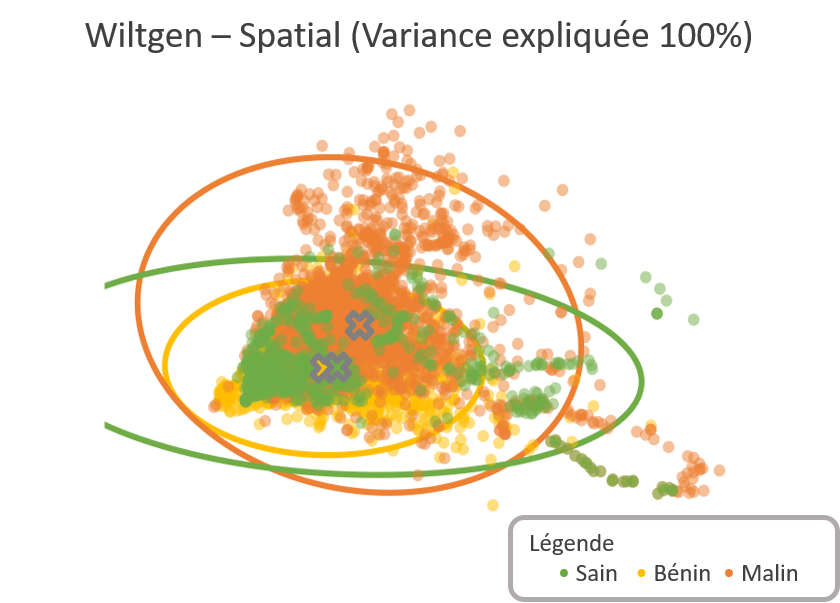
\includegraphics[width=\textwidth]{contents/chapter_4/resources/visualisation_spatial_WiltgenSpatial.png}
    \end{subfigure}
    
    \caption{Visualisation des caractéristiques obtenues par techniques d'extraction spatiales et projection \gls{pca} sur les deux premières composantes.}
    \label{fig:visualisation_spatial}
\end{figure}\par

La \Cref{fig:visualisation_frequency} permet de mettre en évidence la distribution des données extraites par les méthodes d'extraction fréquentielle. Ainsi, les méthodes basées sur l'extraction de caractéristiques de Fourier semblent posséder une distribution similaire quel que soit le nombre de caractéristiques extraites. De plus, la méthode de Fourier proposée par Wiltgen~\cite{Wiltgen2008}, proposant d'extraire des caractéristiques selon diverses directions, ne semble pas influer cette distribution. Du point de vue des méthodes basées sur le principe d'ondelettes, la séparation des données semble être davantage marquée, et l'impact de l'ondelette mère ne semble pas influer sur la distribution des données et des classes. Pour l'ensemble de ces méthodes, les deux premières composantes de l'\gls{pca} semblent suffisantes à exprimer la quasi-intégralité de la variance.\par

\begin{figure}[H]
    \centering
    \begin{subfigure}{.45\textwidth}
      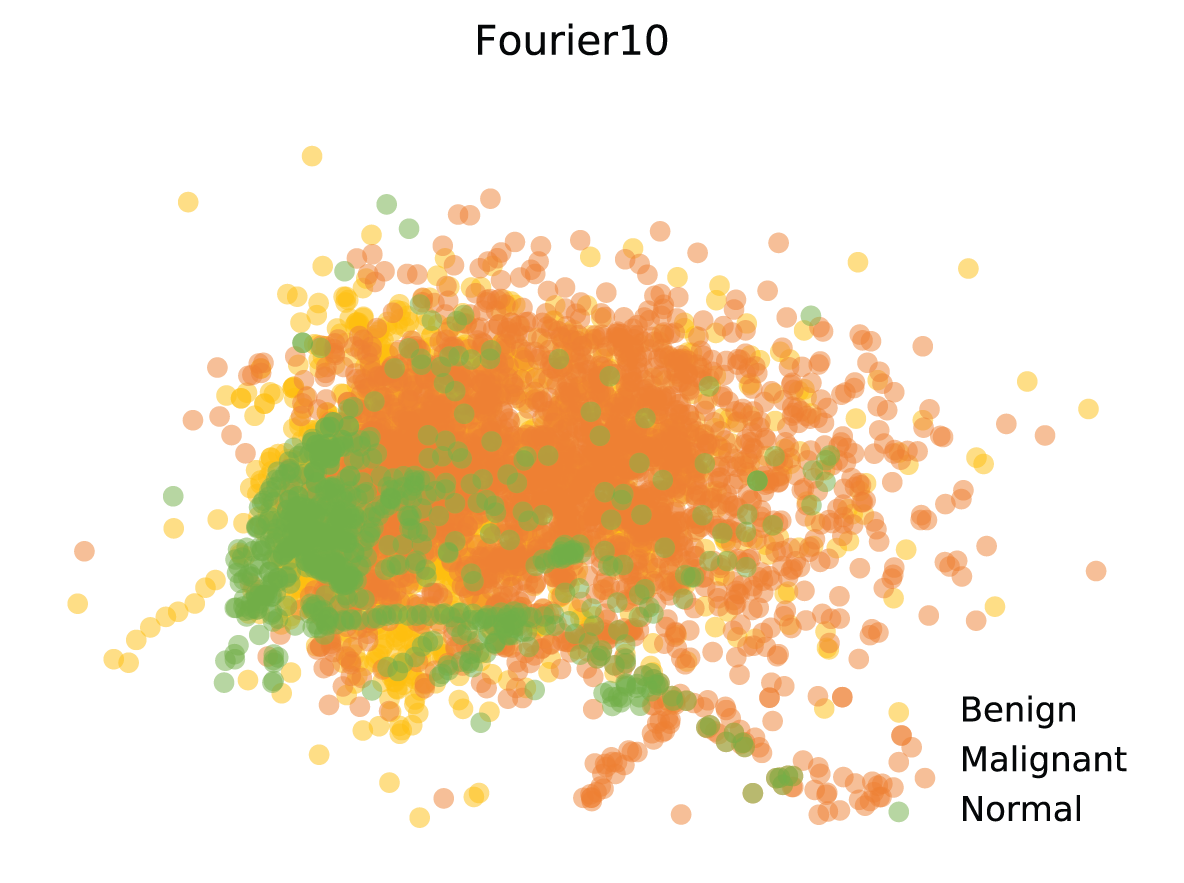
\includegraphics[width=\textwidth]{contents/chapter_4/resources/visualisation_frequency_Fourier10.png}
    \end{subfigure}
    \begin{subfigure}{.45\textwidth}
      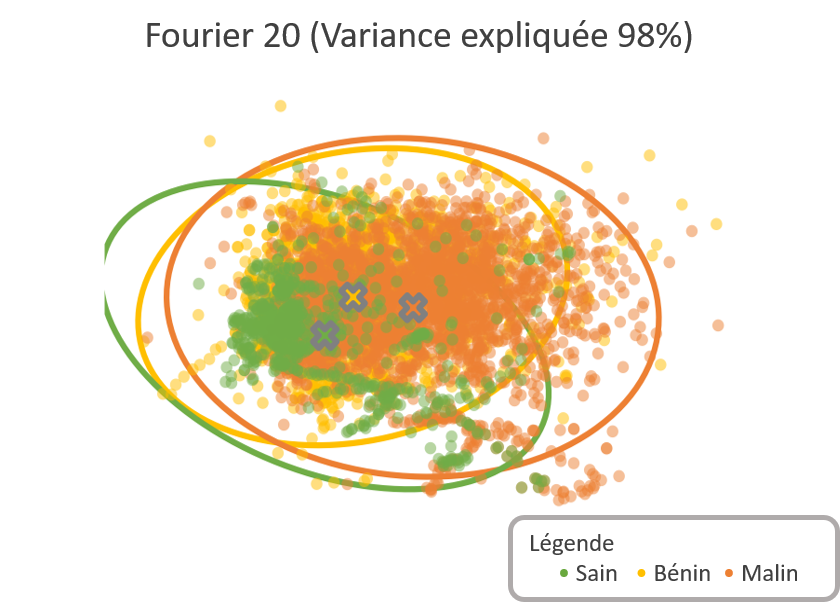
\includegraphics[width=\textwidth]{contents/chapter_4/resources/visualisation_frequency_Fourier20.png}
    \end{subfigure}
    
    \begin{subfigure}{.45\textwidth}
      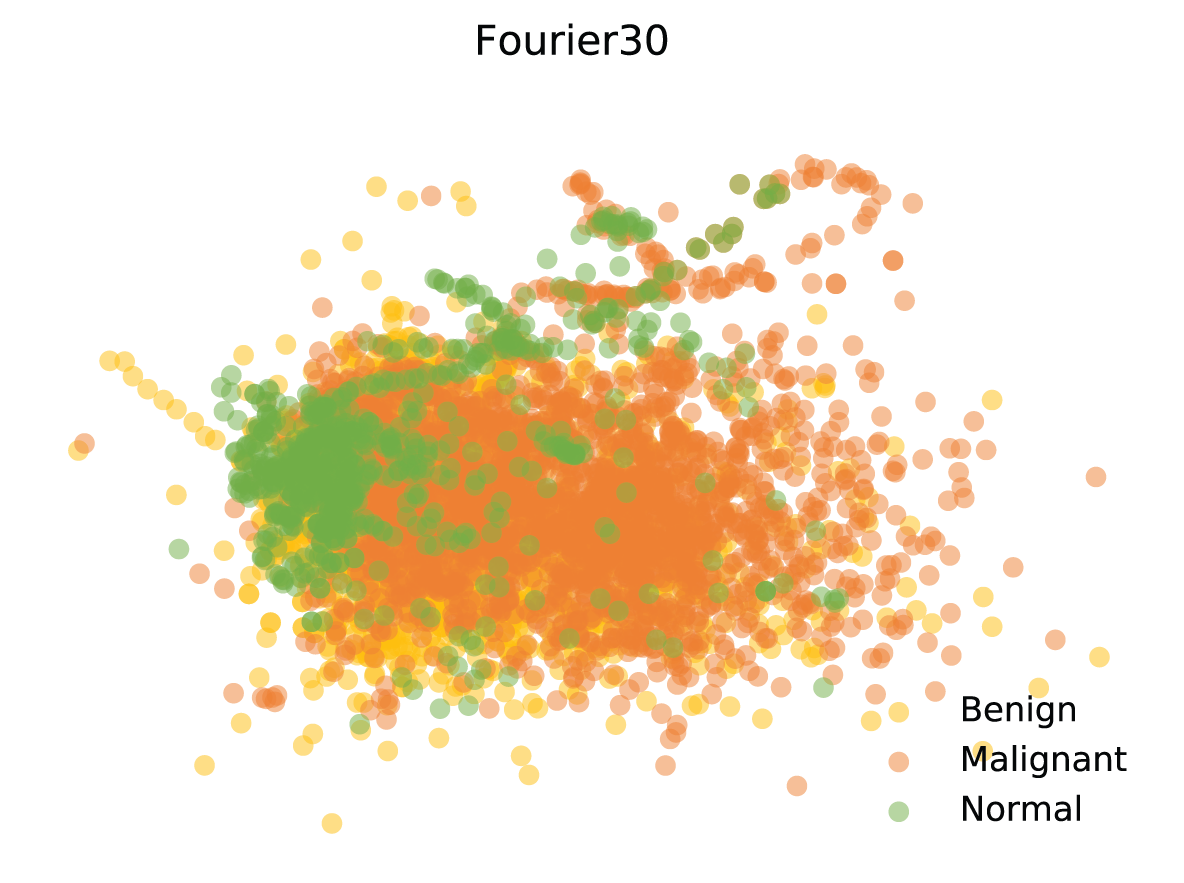
\includegraphics[width=\textwidth]{contents/chapter_4/resources/visualisation_frequency_Fourier30.png}
    \end{subfigure}
    \begin{subfigure}{.45\textwidth}
      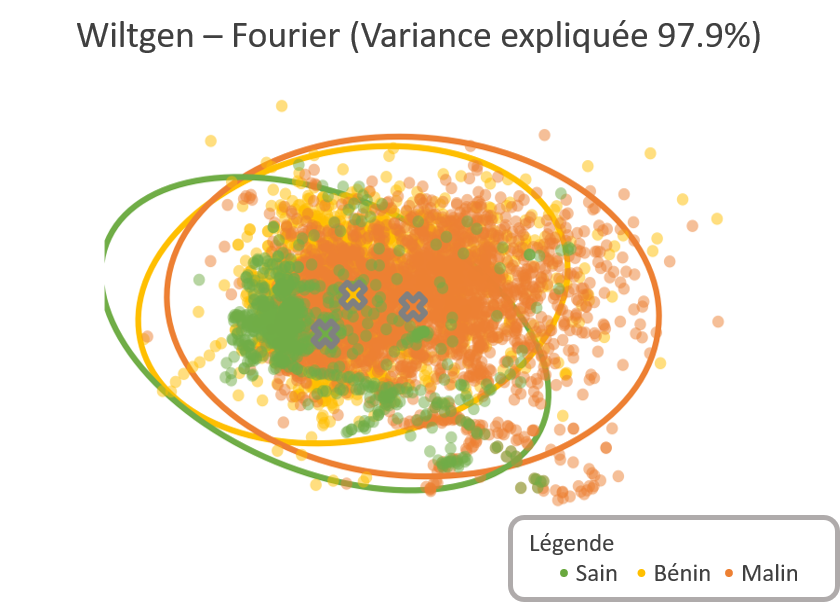
\includegraphics[width=\textwidth]{contents/chapter_4/resources/visualisation_frequency_WiltgenFourier.png}
    \end{subfigure}
    
    \begin{subfigure}{.45\textwidth}
      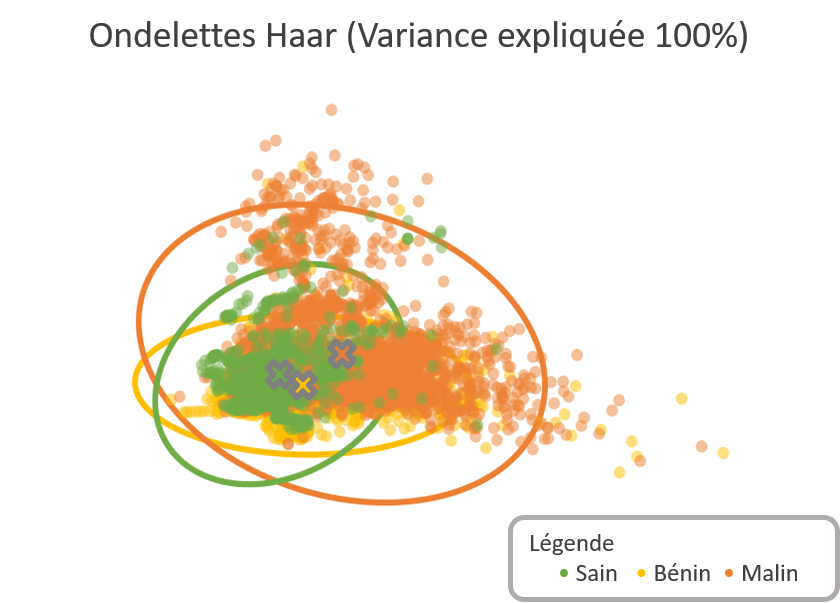
\includegraphics[width=\textwidth]{contents/chapter_4/resources/visualisation_frequency_Haar.png}
    \end{subfigure}    
    \begin{subfigure}{.45\textwidth}
      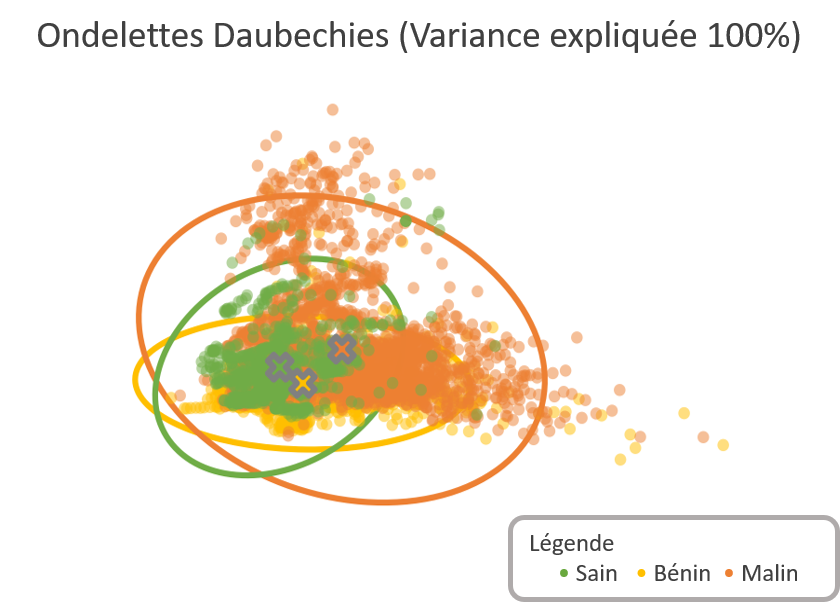
\includegraphics[width=\textwidth]{contents/chapter_4/resources/visualisation_frequency_Daubechies.png}
    \end{subfigure}
    
    \caption{Visualisation des caractéristiques obtenues par techniques d'extraction fréquentielles et projection \gls{pca} sur les deux premières composantes.}
    \label{fig:visualisation_frequency}
\end{figure}\par

Pour finir, la \Cref{fig:visualisation_transfer} recense les projections par \gls{pca} de l'ensemble des méthodes d'extraction basée sur des architecture de \gls{cnn} pré-entraînées, catégorisées sous le terme de transfert par apprentissage. Une différence notable est à remarquer entre les architectures utilisant une couche de global pooling moyen et celle utilisant une couche de global pooling maximum. En effet, la séparation entre classes est marquée de manière plus importante lorsque qu'une couche de global pooling moyen est employé. En addition, cette séparation semble être plus prononcée sur les architectures InceptionV3 et ResNet. Enfin, nous pouvons noter par ces méthodes, que la variance exprimée sur les deux premières composantes n'est que de 20\% à 40\%. Ce dernier constat s'explique par la grande quantité d'information initialement proposé par ces architectures, soit entre 512 et 2048 caractéristiques extraites en comparaison des dizaine d'entre elles extraites par les méthodes manuelles.\par

\begin{figure}[H]
    \centering
    \begin{subfigure}{.45\textwidth}
      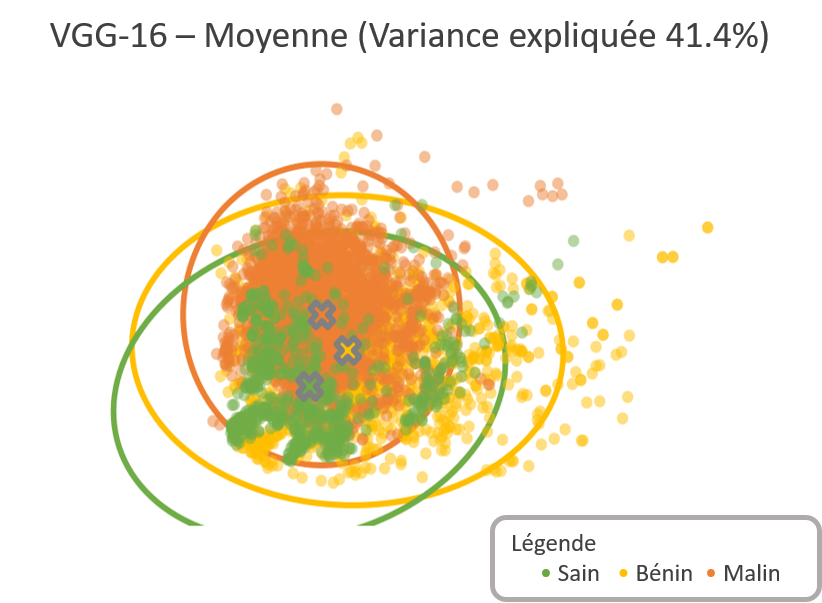
\includegraphics[width=\textwidth]{contents/chapter_4/resources/visualisation_transfer_VGG16Avg.png}
    \end{subfigure}
    \begin{subfigure}{.45\textwidth}
      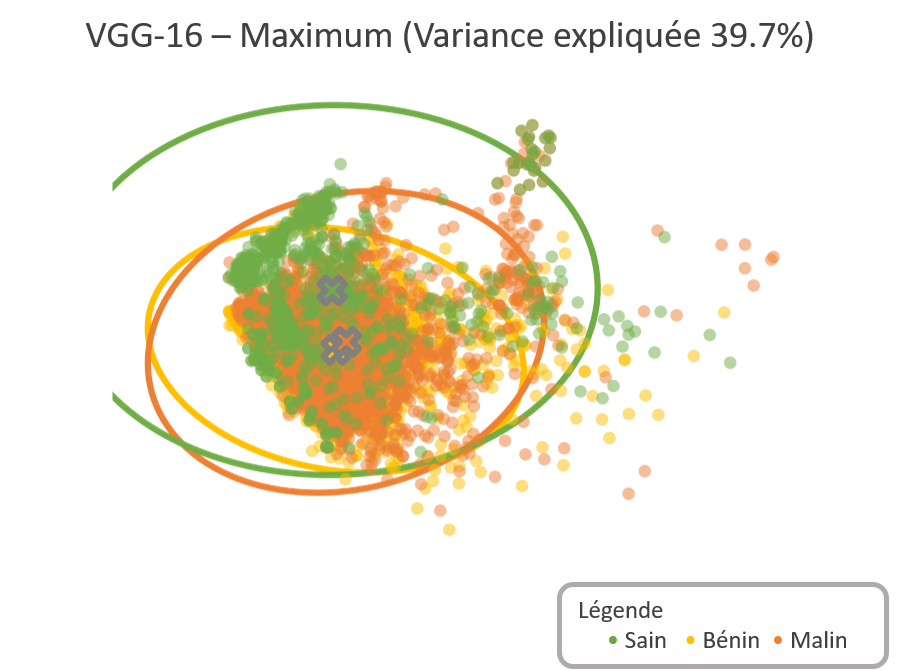
\includegraphics[width=\textwidth]{contents/chapter_4/resources/visualisation_transfer_VGG16Max.png}
    \end{subfigure}
    
    \begin{subfigure}{.45\textwidth}
      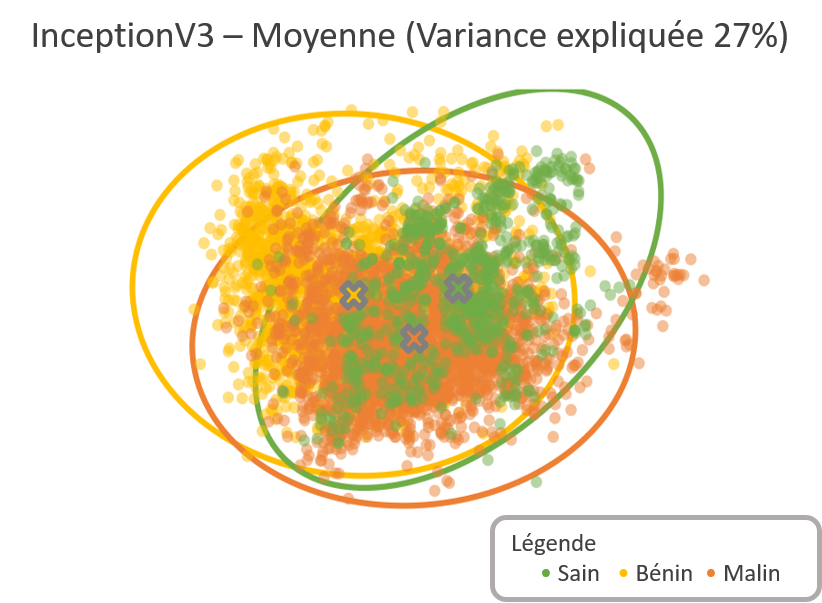
\includegraphics[width=\textwidth]{contents/chapter_4/resources/visualisation_transfer_InceptionV3Avg.png}
    \end{subfigure}
    \begin{subfigure}{.45\textwidth}
      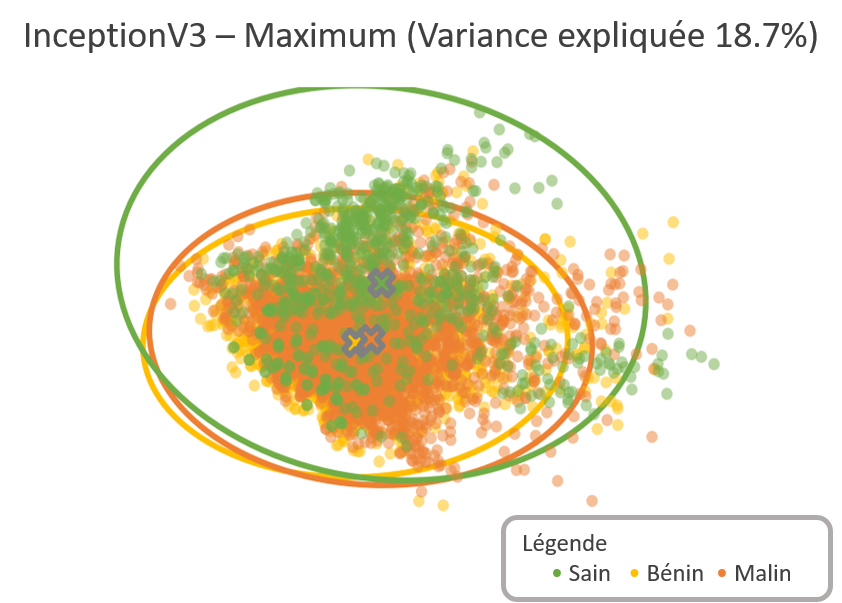
\includegraphics[width=\textwidth]{contents/chapter_4/resources/visualisation_transfer_InceptionV3Max.png}
    \end{subfigure}
    
    \begin{subfigure}{.45\textwidth}
      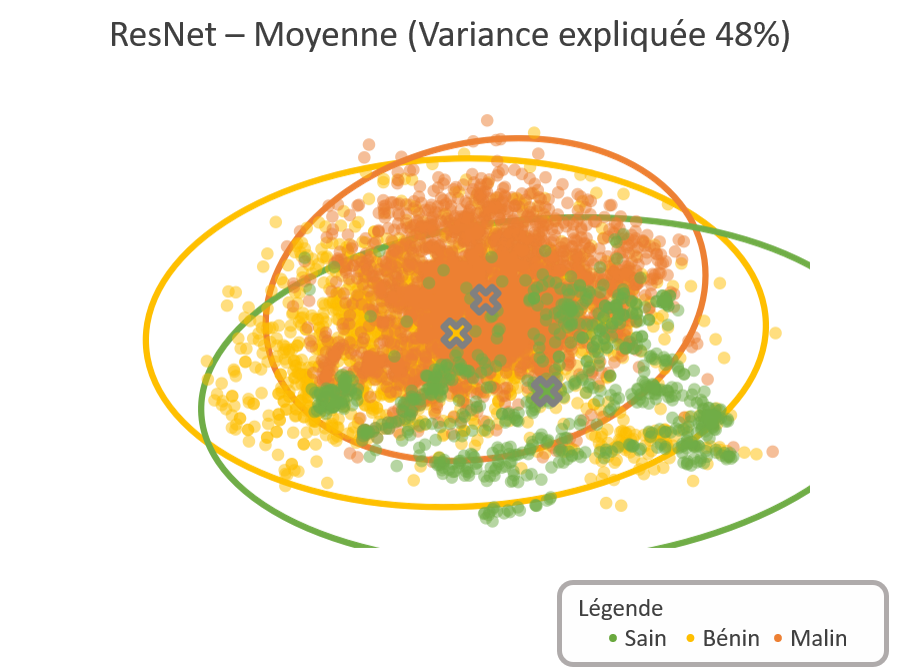
\includegraphics[width=\textwidth]{contents/chapter_4/resources/visualisation_transfer_ResNetAvg.png}
    \end{subfigure}
    \begin{subfigure}{.45\textwidth}
      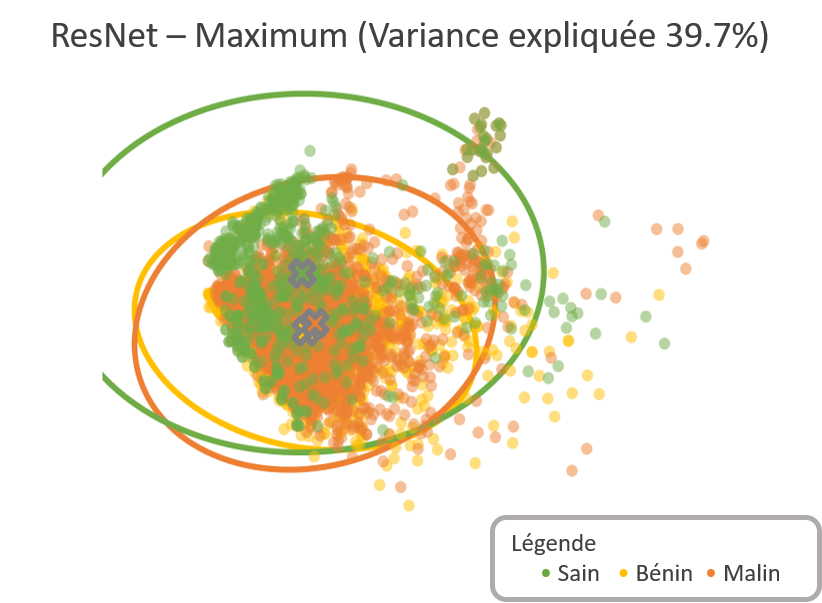
\includegraphics[width=\textwidth]{contents/chapter_4/resources/visualisation_transfer_ResNetMax.png}
    \end{subfigure}
    
    \begin{subfigure}{.45\textwidth}
      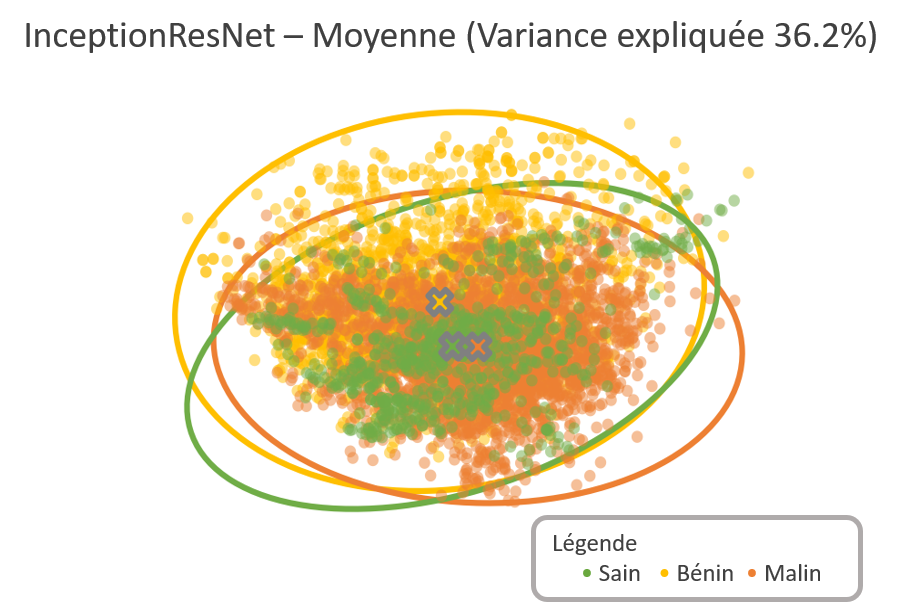
\includegraphics[width=\textwidth]{contents/chapter_4/resources/visualisation_transfer_InceptionResNetAvg.png}
    \end{subfigure}
    \begin{subfigure}{.45\textwidth}
      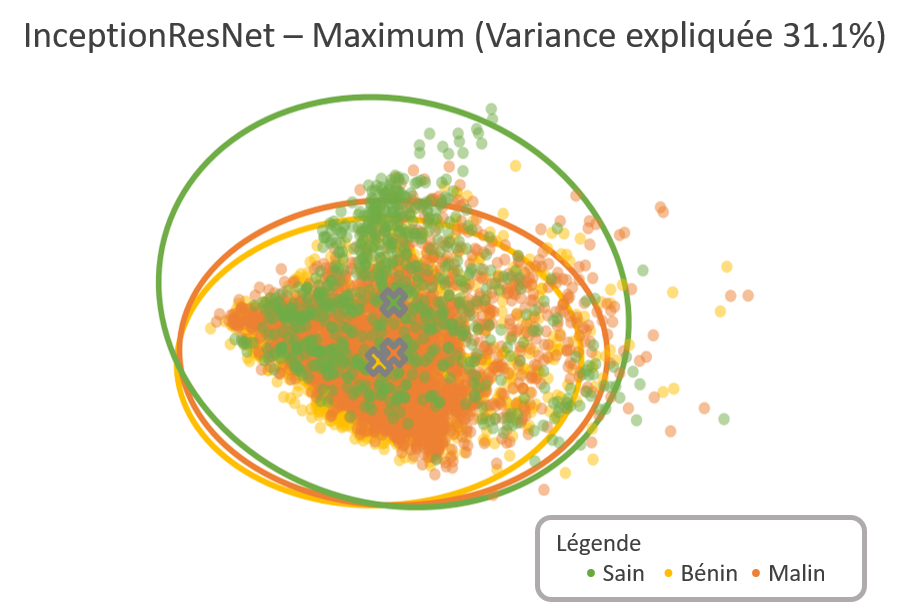
\includegraphics[width=\textwidth]{contents/chapter_4/resources/visualisation_transfer_InceptionResNetMax.png}
    \end{subfigure}
    
    \caption{Visualisation des caractéristiques obtenues par techniques d'extraction basées sur des réseaux de type \gls{cnn} pré-entraînés sur la base ImageNet et projection \gls{pca} sur les deux premières composantes.}
    \label{fig:visualisation_transfer}
\end{figure}\par

\clearpage


%%%%%%%%%%%%%%%%%%%%%%%%%%%%%%%%%% 
%%%%%%%%%%%%%%%%% PRE TRAITEMENTS
\section{Pré-traitements de caractéristiques}
Cette partie dédiée au pré-traitement de caractéristiques, se consacre à l'ensemble des transformations opérées après extraction de l'information par le biais des techniques évoquées en \Cref{chap:feature_extraction}. Nous aborderons au sein de cette section les diverses solutions à notre disposition pouvant parfaire la classification de notre problématique. En effet, de nombreuses contraintes peuvent affecter le bon déroulement de la classification~:
\begin{itemize}
    \item un déséquilibre au sein des annotations des divers types de tissus a séparé bien que celui-ci ait été minimisée,
    \item un nombre de caractéristiques trop important conduisant à du sur-apprentissage ou des difficultés à séparer le problème (voir l'extraction de caractéristiques par \gls{cnn}),
    \item ou encore une information non consistante.
\end{itemize}\par

Ainsi, cette partie tentera de répondre à ces questions à l'aide de différents domaines d'étude visant à corriger tout ou partie de ces éléments et nous les aborderons d'un point de vue logique en termes de processus de classification. Ainsi et dans un premier temps, nous discuterons de la \textbf{normalisation} des caractéristiques et de son intérêt au sein de processus de classification. Dans un second temps, nous traiterons des techniques de \textbf{réduction de l'information} et proposerons des solutions notamment dans le cadre de l'extraction de caractéristiques par \gls{cnn}. Finalement, nous aborderons le \textbf{balancement de données} et les principales stratégies mises à disposition.

\subsection{Réduction de dimensions}
Dans le domaine de l'apprentissage automatique, la réduction de dimension est une technique qui permet de diminuer le nombre de dimensions afin de rendre un problème moins complexe, tout en conservant une information suffisante à la résolution du problème. Également, elle est un moyen de se prévenir du "Fléau de la dimension", phénomène qui met en perspective d'une part la croissance exponentielle de l'ajout de nouvelles dimensions à la dilution des divers échantillons dans cet espace. Ce dilemme a pour principales conséquences d'augmenter la complexité d'un problème, la durée nécessaire à sa résolution mais également d'engendrer des risques de sur-apprentissage.\par

Les caractéristiques extraites par méthode spatiales et fréquentielles étant assez restreintes (respectivement de 14 à 56 variables et, de 10 à 39 variables), nous n'étudierons pas leur impact sur ces méthodes. En revanche, le nombre des caractéristiques extraite par méthode de transfert de connaissance est important et varient de 512 à 2048 variables. Nous évaluerons l'impact de certaines d'entre elles sur ces cas particuliers.\par

A cette fin, deux catégories de méthodes cohabitent~: d'une part les méthodes de sélection de caractéristiques qui réduisent l'espace en décimant certaines dimensions jugées non pertinente à la résolution du problème ; d'autre part les méthodes par projection ou transformation de l'espace existant qui réduisent et modifient les valeurs existantes. Dans la mesure où nous emploierons cette technique dans le cadre de l'apprentissage par transfert de connaissance, notre investigation ne portera que sur cette seconde catégorie de méthodes. En effet, les méthodes par sélection de caractéristiques ne nous semblent pas pertinente dans le cadre de caractéristiques auto déterminées par des réseaux profonds.\par

L'\gls{pca} est l'une de ces techniques, dont l'idée majeure est de retirer l'information redondante pour ne conserver que l'information de variance, supposée contenir l'information. Cette méthode cherche ainsi à identifier les axes selon lesquels la variation des données est maximisée. Il sera ensuite nécessaire de déterminer un nombre d'axes suffisant à séparer le problème (réduction du nombre de caractéristiques). Plutôt que de choisir ce nombre arbitraire, la littérature préfère retenir des seuils pertinents de cette variance, les plus communs sont 95\%, 97.5\% et 99\%.\par

Le \gls{lda} est une seconde technique employée à une fin de réduction de l'information, pour laquelle nous recherchons des axes de projection qui maximisent la variance inter-groupe. Pour comparaison, la variance est le résultat de la somme de la variance intra-groupe et inter-groupe. De la même manière, nous retiendrons des seuils similaires à ceux de l'\gls{pca} soit 95\%, 97.5\% et 99\%.\par

La \Cref{tab:summary_reduction_methods} permet de résumer ces méthodes et paramétrage associés que nous évaluerons.\par 

\begin{table}[H]
    \centering
    \begin{tabular*}{0.6\linewidth}{lll}
        \toprule
        \textbf{Méthode}       & \textbf{Paramètre}                 & \textbf{Valeurs}                      \\ \midrule
        \gls{pca}              & \multirow{2}{*}{Variance expliquée}& \multirow{2}{*}{[0.95, 0.975, 0.99]}  \\ \cline{1-1}
        \gls{lda}              &                                    &                                       \\ 
        \bottomrule
    \end{tabular*}
    \caption{Liste des méthodes de réduction employées et leurs paramètres associés.}
    \label{tab:summary_reduction_methods}
\end{table}\par

\subsection{Normalisation de caractéristiques}
\label{subsec:features_normalisation}
Selon le domaine d'étude visée, la normalisation de caractéristiques peut être l'une des étapes cruciales quant au bon déroulement de ce processus de classification. Notre recherche a été amenée à considérer cet aspect suite à la dégradation des résultats d'un travail proche de notre thématique portant sur la classification d'image de dermatoscopie~\cite{Celebi2007}.\par

Il est communément admis que des méthodes tels que les \gls{knn} dont le principe repose sur des critères de distances, peuvent être fortement affectés par des caractéristiques non normalisées. Pour d'autres méthodes de classification, cette normalisation des caractéristiques fait davantage appel à un bon sens vis-à-vis de leur principe de fonctionnement. Nous noterons le retour de certains travaux sur la dégradation des performances sur les \gls{svm}~\cite{Juszczak2002} mais également les réseaux de neurones~\cite{Celebi2007}.\par

Diverses méthodes ont ainsi été proposées afin de remédier à ces défauts de distribution de l'information. L'un de ces travaux propose de réduire l'erreur de classification de modèles \gls{svm} par l'apport de normalisations tenant compte de la variance, du maximum ou encore conjointement du minimum et du maximum~\cite{Juszczak2002}. Le travail mené par Celebi et al.~\cite{Celebi2007} propose une normalisation des caractéristiques à l'aide de la "Cote Z" ou "Standard score", c'est à dire par soustraction de la moyenne au sein d'un même groupe de caractéristiques puis par division de l'écart type de ce même groupe.\par

Afin de couvrir au mieux cette problématique de la normalisation, nous l'aborderons à l'aide des deux méthodes majeure de ces deux précédentes études, dont l'\Cref{eq:scaling_methods} reprend les expressions sous forme mathématique. Ainsi, nous envisagerons l'utilisation de~:
\begin{itemize}
    \item la normalisation par "Mininimum et Maximum"~\cite{Juszczak2002},
    \item et de la normalisation "Standard" ou "Cote Z"~\cite{Celebi2007}.
\end{itemize}\par

\begin{equation} 
    \label{eq:scaling_methods}
    \begin{split}
    &MinMax=\frac{X-min(X)}{max(X)-min(X)}  \\
    &Standard=\frac{X-\mu{}}{\sigma}	    
    \end{split}
\end{equation}

\subsection{Balancement de données}
L'une des problématiques associées de manière récurrente à l'apprentissage sur des données réelles est celle de la répartition homogène des annotations, en opposition aux domaines impliquant des données synthétiques pouvant provenir de modèles génératifs par exemple. Ces déséquilibres d'annotations sont qualifiés sous le terme anglophone de "class imbalance"~\cite{Prati2009, He2009}.\par

Ces déséquilibres sont propres à de nombreux domaines d'applications, mais touchent essentiellement des champs d'activités dans lesquels la tâche visée correspond à la détection d'événements isolés au sein d'une population, comme par exemple~: 
\begin{inlinerate}
    \item les comportements déviants (fraude bancaire~\cite{Phua2004}),
    \item le respect de critère de qualité (vérification de pièces industrielles~\cite{Wu2018}),
    \item ou encore d'anormalités clinique (cancers ou d'autres pathologies cliniques~\cite{Celebi2007}).
\end{inlinerate}\par

Certains choix peuvent permettre de limiter l'impact d'un déséquilibre d'annotations. Ainsi, la sélection d'un métrique adéquate peut permettre de limiter la dépendance au données~: la substitution de la précision par des mesures telles que l'\gls{auc}~\cite{Celebi2007} ou le \fscore{} sont des solutions pertinentes dans de telles situations. Néanmoins, la plupart des modèles de classification échoueront à classifier convenablement les données dans des situations de forts déséquilibres. Ces modèles préférerons prédire constamment la classe majoritaire, pour minimiser le coût de l'erreur~\cite{Huang2013}. Dans le cadre de modèles basés sur des arbres de décision, la stratégie générale propose de déterminer les critères majeurs de séparation par partitionnement successif des données. Ce partitionnement conduit inéluctablement à un affaiblissement des classes minoritaires~\cite{He2009}. Deux catégories d'approches coexistent pour solutionner ces déséquilibres~\cite{Huang2013}, d'une part les approches par augmentation ou décimations des diverses catégories d'annotation, et d'autres part les approches algorithmiques consistent à pondérer la valeur des annotations afin de prendre en considération le déséquilibre de l'information~\cite{Ting2002,He2009,Thai2010}.\par

En premier lieu, des approches par correction des données simples, proposes diverses solutions pour palier à ces déséquilibres de classes~\cite{Prati2009, He2009}. Une première catégorie de ces méthodes consiste à \textbf{sous-échantillonner} les données jusqu'à obtenir une égalité entre les classes. Son principe le plus simple est celui du "Sous-échantillonnage aléatoire" consistant à décimer de manière aléatoire les données des classes majoritaires afin d'égaler les échantillons de la classe minoritaire. A l'inverse, une autre catégorie consiste à \textbf{sur-échantillonner} les données possédées afin d'obtenir à nouveau une égalité entre classes. Le principe le plus simples est celui du "Sur-échantillonnage aléatoire" consistant à dupliquer aléatoirement les échantillons des classes minoritaires afin d'égaler le nombre d'élément de la classe majoritaire. Le schéma en \Cref{fig:scheme_data_balancing} reprendre l'idée de ces deux principes.\par

En second lieu, des approches par correction des données plus avancées ont été proposées. De manière non exhaustive nous proposerons l'une d'entre elle pour chaque catégorie~:
\begin{itemize}
    \item par \textbf{sous-échantillonnage}~: cette catégorie consiste à décimer le nombre d'échantillons à celle de la classe minoritaire. Nous considérerons une décimation des échantillons aléatoire pour cette catégorie.
    \item par \textbf{sur-échantillonnage}~: cette catégorie consiste à augmenter les éléments des classes minoritaires. Nous considérerons une duplication aléatoire de ces éléments.
    \item par \textbf{combinaison}~: cette catégorie consiste à mêler des méthodes propres aux deux précédentes catégories. L'utilisation de méthode \gls{smote}~\cite{Chawla2002}  est alors réalisé dans un premier temps pour générer de manière synthétique de nouveaux éléments, puis la méthode \gls{tl}~\cite{Tomek1976} ou \gls{enn} est utilisée pour enlever les incohérences des éléments originaux ou synthétiques.
\end{itemize}\par

\begin{figure}[H]
    \centering
    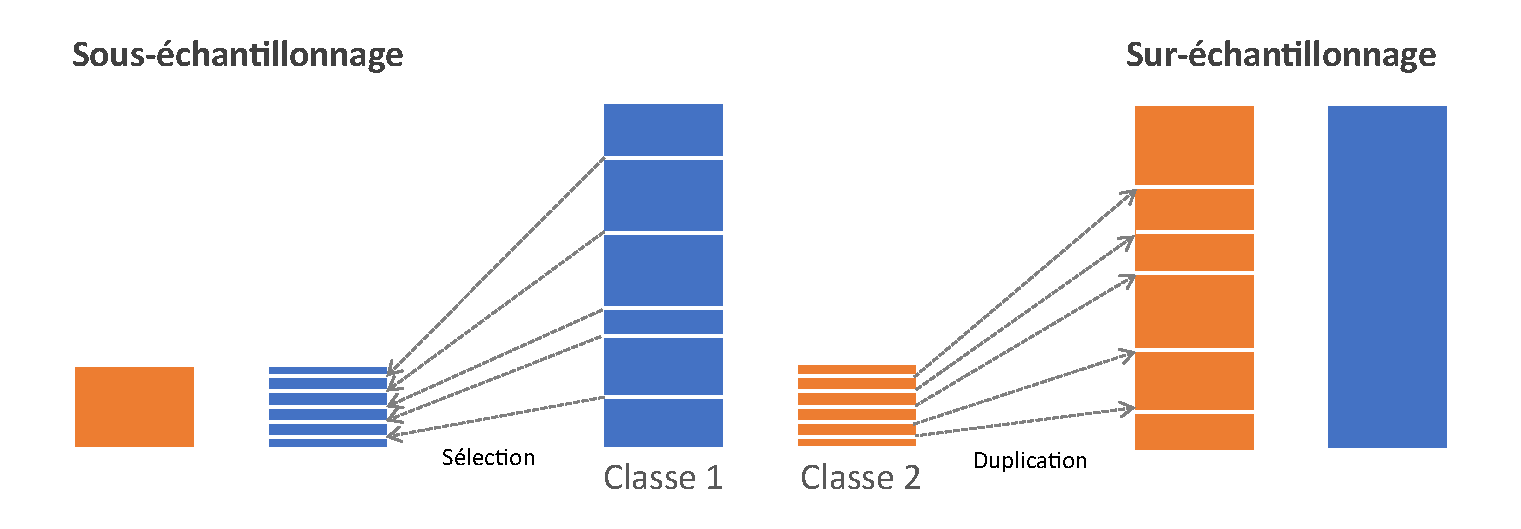
\includegraphics[width=\linewidth]{contents/chapter_4/resources/scheme_data_balancing.pdf}
    \caption{Schéma des deux stratégies principales de balancement de données. A gauche, la stratégie de sous-échantillonnage, dans laquelle des éléments sont aléatoirement choisis jusqu'à réduire l'ensemble des classes au nombre d'éléments de la classe minoritaire ; A droite, la stratégie de sur-échantillonnage, dans laquelle les éléments des classes minoritaires sont dupliqués aléatoirement. }
    \label{fig:scheme_data_balancing}
\end{figure}\par

En opposition à ces méthodes dédiées, les approches par pondération des échantillons consistent à gérer le déséquilibre des annotations en appliquant des poids d'importance différente selon la provenance échantillon lors de l'apprentissage du modèle. Nous considérerons ce choix par défaut, puisqu'il permet de contrer de manière assez intuitive ces

Dans l'optique de récapituler cette partie, les méthodes utilisées dans le but de corriger le déséquilibre des données sont référencée dans la \Cref{tab:summary_balancement_methods}. Afin de traiter au mieux cette tâche, le balancement de données par ses différentes stratégies évoquées est réalisé avec l'aide de la librairie logicielle "Imbalanced-learn"~\cite{Lemaitre2017}. La correction par algorithme, plus précisément pondération, sera réalisé avec l'aide de la bibliothèque "Scikit-learn"~\cite{pedregosa2011}.\par

\begin{table}[H]
    \centering
    \begin{tabular*}{0.6\linewidth}{l@{\extracolsep{\fill}}l}
        \toprule
        \textbf{Catégorie}                  & \textbf{Méthode}      \\ \hline
        Sous-échantillonnage                 & Aléatoire             \\ \hline
        Sur-échantillonnage                  & Aléatoire             \\ \hline
        \multirow{2}{*}{Combinaison}        & SMOTE + Tomek         \\ \cline{2-2}
                                            & SMOTE + EN            \\
        \bottomrule
    \end{tabular*}
    \caption{Liste des diverses méthodes de balancement mises en œuvre pour corriger les déséquilibre de données.}
    \label{tab:summary_balancement_methods}
\end{table}\par

\section{Méthodes de prédiction}
Afin d'œuvrer à la séparation des échantillons en notre possession sur la base de leurs caractéristiques, nous aurons recours à divers modèles de classification, dont nous évaluerons les performances de classification. En effet, bien que les avantages et inconvénients de la plupart d'entre eux aient été évoqués au sein de la \Cref{sec:models_settings}, nous n'avons pas de contraintes de rapidité lors de la phase d'apprentissage ou de prédiction. Seules les performances de classifications seront mesurées dans ce travail.\par

\begin{table}[H]
    \centering
    \begin{tabular}{cll}
        \toprule
        \textbf{Modèle}                                 & \textbf{Hyperparamètres}  & \textbf{Valeurs}                          \\ \midrule
        \multirow{4}{*}{\gls{cart}}                     & Profondeur maximum        & [3, $\infty$]                             \\ \cmidrule{2-3} 
                                                        & Critère de qualité        & [Gini, Entropie]                          \\ \cmidrule{2-3}   
                                                        & Caractéristiques maximum  & [1, 2, 3, 4, 5, 6, 7, 8, 9]               \\ \cmidrule{2-3}   
                                                        & Échantillons minimum      & [1, 2, 3, 4, 5, 6, 7, 8, 9]               \\ \midrule 
        \multirow{4}{*}{\gls{rf}}                       & Profondeur maximum        & [3, $\infty$]                             \\ \cmidrule{2-3} 
                                                        & Critère de qualité        & [Gini, Entropie]                          \\ \cmidrule{2-3}   
                                                        & Caractéristiques maximum  & [1, 2, 3, 4, 5, 6, 7, 8, 9]               \\ \cmidrule{2-3}   
                                                        & Échantillons minimum      & [1, 2, 3, 4, 5, 6, 7, 8, 9]               \\ \midrule 
        \multirow{4}{*}{\gls{gb}}                       & Profondeur maximum        & [3, $\infty$]                             \\ \cmidrule{2-3}
                                                        & Critère                   & [MSE, MAE]                                \\ \cmidrule{2-3} 
                                                        & Caractéristiques maximum  & [1, 2, 3, 4, 5, 6, 7, 8, 9]               \\ \cmidrule{2-3}   
                                                        & Échantillons minimum      & [1, 2, 3, 4, 5, 6, 7, 8, 9]               \\ \midrule 
        \gls{svm} - Noyau linéaire                      & C                         & [0.001, 0.01, 0.1, 1, 10, 100, 1000]      \\ \midrule
        \multirow{2}{*}{\gls{svm} - Noyau RBF}          & C                         & [0.001, 0.01, 0.1, 1, 10, 100, 1000]      \\ \cmidrule{2-3}   
                                                        & Gamma                     & [0.001, 0.01, 0.1, 1, 10, 100, 1000]      \\ \midrule 
        \multirow{5}{*}{\gls{mlp}}                      & Couche cachées            & [(20,), (20,20,), (20,20,20,)]            \\ \cmidrule{2-3}
                                                        & Activation                & [Tanh, ReLu]                              \\ \cmidrule{2-3}
                                                        & Solveur                   & [SGD, Adam]                               \\ \cmidrule{2-3}
                                                        & Alpha                     & [0.001, 0.01, 0.1, 1, 10, 100, 1000]      \\ \cmidrule{2-3}
                                                        & Taux d'apprentissage      & [Constant, Adaptatif]                     \\ \bottomrule 
    \end{tabular} 
    \caption{Table recensant l'ensemble des modèles de classification et leurs hyperparamètres évalués lors des expériences que nous mènerons.}
    \label{tab:image_classification_models_hyperparameters}
\end{table}\par

Dans un premier temps, nous évaluerons nos données à l'aide de \gls{cart} dont l'utilité a été démontré par l'un de nos travaux de référence ~\cite{Wiltgen2008}. Néanmoins, ces modèles tendent au sur-apprentissage dans des contextes où les dimensions sont nombreuses, ainsi nous évaluerons de manière complémentaires les \gls{rf}~\cite{Breiman2001} et les \gls{gb} plus aptes à gérer cet aspect. Dans un second temps, nous envisageons les modèles \gls{svm} employés dans de nombreux contextes de classification~\cite{Smach2008a}, mais également de classification de lésion de la peau~\cite{Celebi2007}. Enfin, nous envisagerons la piste des \gls{mlp} afin de d'évaluer notre problématique de manière non linéaire.\par

Afin d'évaluer au mieux chacun de ces modèles, nous affinerons les hyperparamètres majeurs de chacun de ces modèles. Il sera bien entendu nécessaire de faire des compromis dans le choix de ces valeurs, et opterons pour celles les plus couramment utilisées. L'ensemble des modèles de classification et de leurs hyperparamètres et valeurs associés sont recensés sur la \Cref{tab:image_classification_models_hyperparameters}.\par

\section{Processus et métriques}
Pour réaliser l'évaluation, nous emploierons une validation croisée imbriquée déjà discuté sur le \Cref{sec:models_settings}. Cette structure de validation a été choisie car moins sujet au biais~\cite{Cawley2010}, de plus une valeur de $k$ comprise entre 5 et 10 pour l'évaluation est démontré empiriquement comme un bon compromis entre biais et variance~\cite{James2000}. Les expériences de ce chapitre sont réalisée avec une valeur $k$ de quatre pour l'évaluation afin de réduire la durée de calcul à un temps raisonnable et de deux lots pour la validation, leurs combinaison représentant un bon compromis vis-à-vis de nos expériences. Ces répartitions sous forme de lot de nos données est visible sur la \Cref{fig:visualisation_folds}.\par

\begin{figure}[H]
    \centering
    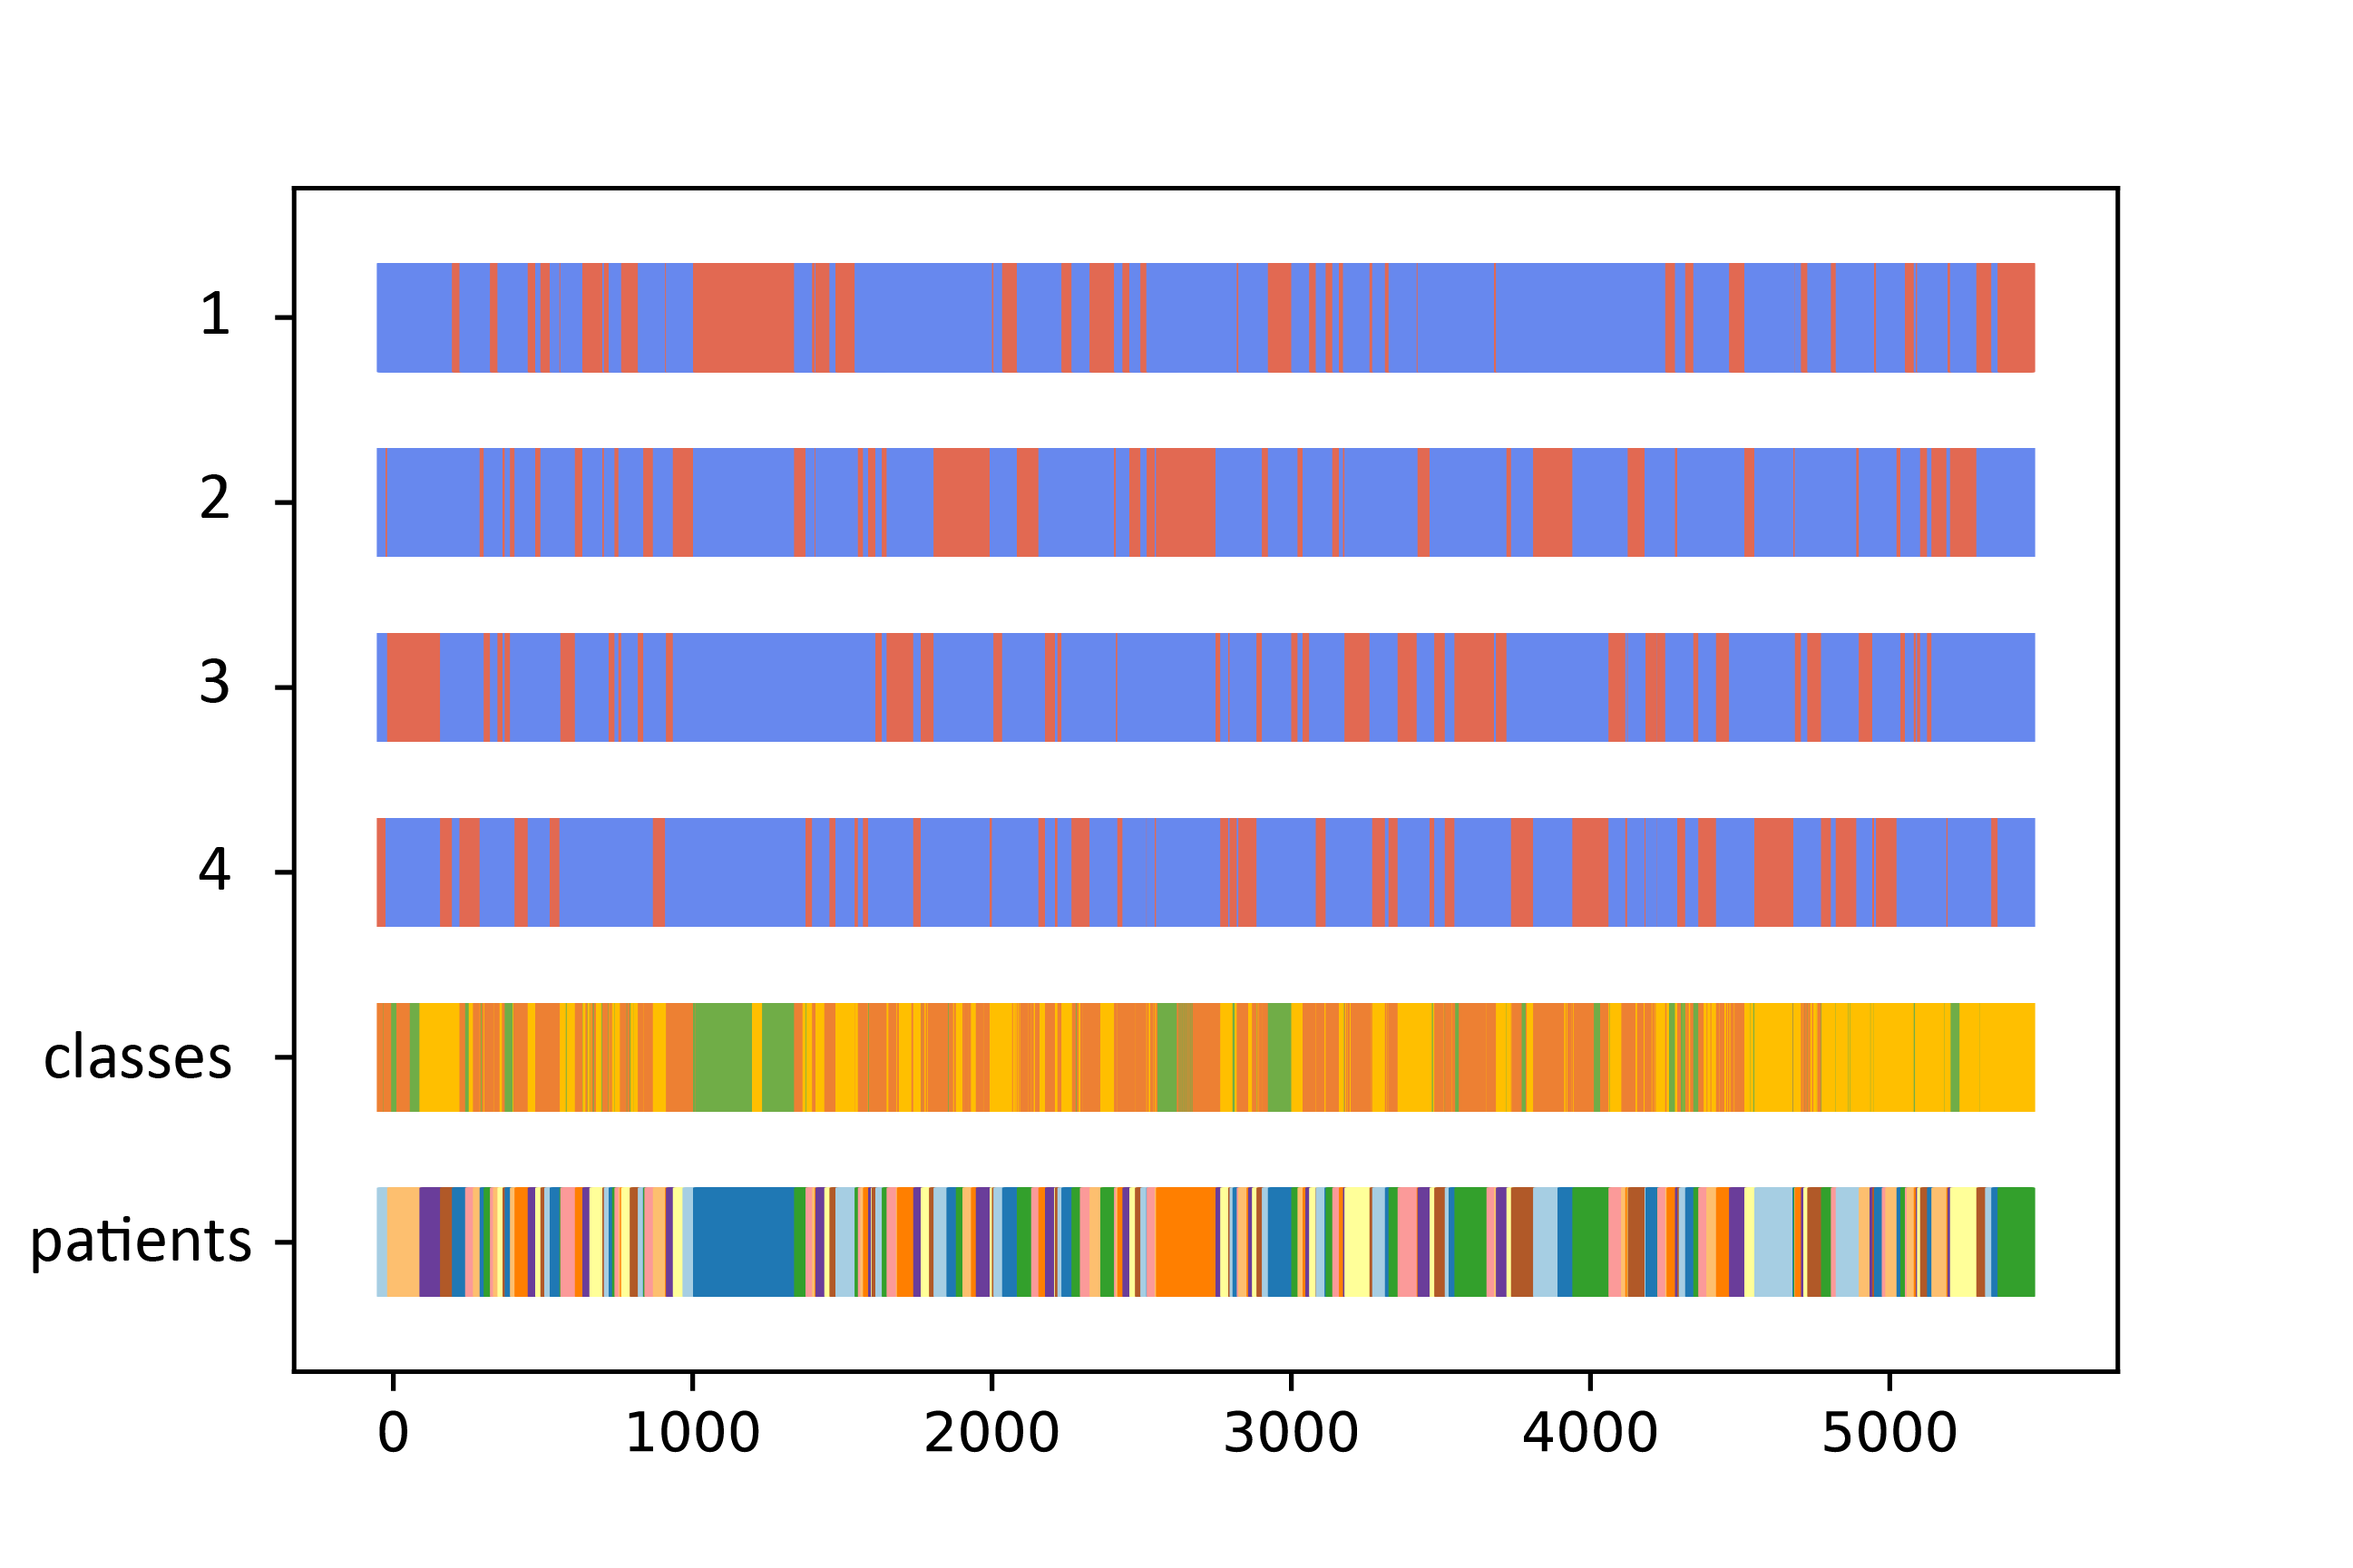
\includegraphics[width=0.7\linewidth]{contents/chapter_4/resources/visualisation_folds.png}
    \caption{Visualisation des divers lots d'évaluation utilisés pour l'évaluation des processus de classification.}
    \label{fig:visualisation_folds}
\end{figure}\par

Afin de régler les hyperparamètres et d'évaluer les performances des divers modèles, nous opterons pour un métrique de type \fscore{} également discuté durant le \Cref{sec:models_settings}. En effet, cette métrique est robuste face à des déséquilibres d'annotations, et représente conjointement sous une unique mesure la précision ainsi que le rappel. Son expression est binaire, il sera ainsi calculé pour chaque classe dont nous pondérerons la valeur par le ratio du nombre de d'échantillons disponibles pour chacune d'entre elles.\par

Ces expériences seront menées en plusieurs étapes successives, et nous débuterons par l'évaluation de l'ensemble des méthodes d'extraction de caractéristiques conjointement à la normalisation de l'information selon le Minimum/Maximum et Standard. Aucun de ces tests ne sera mené sur les caractéristiques brutes, les modèles ne convergeant pas dans un temps raisonnable selon le modèle employé.\par

Dans une seconde phase, nous mesurerons l'impact de la réduction de dimension sur les techniques de transfert de connaissance avant de procéder à leur classification. Contrairement aux recommandations de la librairie~\textsuperscript{\ref{footnote:exemple_pca_scaling}}, nous opterons pour un schéma de type réduction de l'information puis de normalisation de caractéristiques avant classification. En effet, les caractéristiques issues de réseaux convolutionnels possèdent une distribution de valeurs consistantes, et n'affectent pas de manière significative les techniques de réduction de dimensions. En revanche, la réduction d'information par techniques de projection peut affecter la consistance de cette distribution des valeurs. Ce phénomène a notamment été observé sur un lot de 500 données choisies arbitrairement, et présentée sur la \Cref{fig:visualisation_scaling_reduction}.\par

Pour finir ces expériences, nous finirons par mesurer l'impact du balancement des données sur les résultats de classification et évaluerons l'utilité des techniques qui visent à corriger ce déséquilibre.\par

Les choix que nous réaliserons entre ces diverses étapes se baseront sur les résultats à trois classes dans la mesure où ces scores seront représentatifs de la capacité à caractériser la problématique dans son ensemble. Néanmoins dans la dernière partie de cette analyse, nous considérerons les résultats de la détection des images malignes, principal objectif visé par ce travail.\par

\addtocounter{footnote}{1}
\footnotetext[\thefootnote]{Source~: Scikit-learn - \href{https://scikit-learn.org/stable/auto_examples/preprocessing/plot_scaling_importance.html}{"Importance of Feature Scaling"}. \label{footnote:exemple_pca_scaling}}
 
\begin{figure}[H]
    \centering
    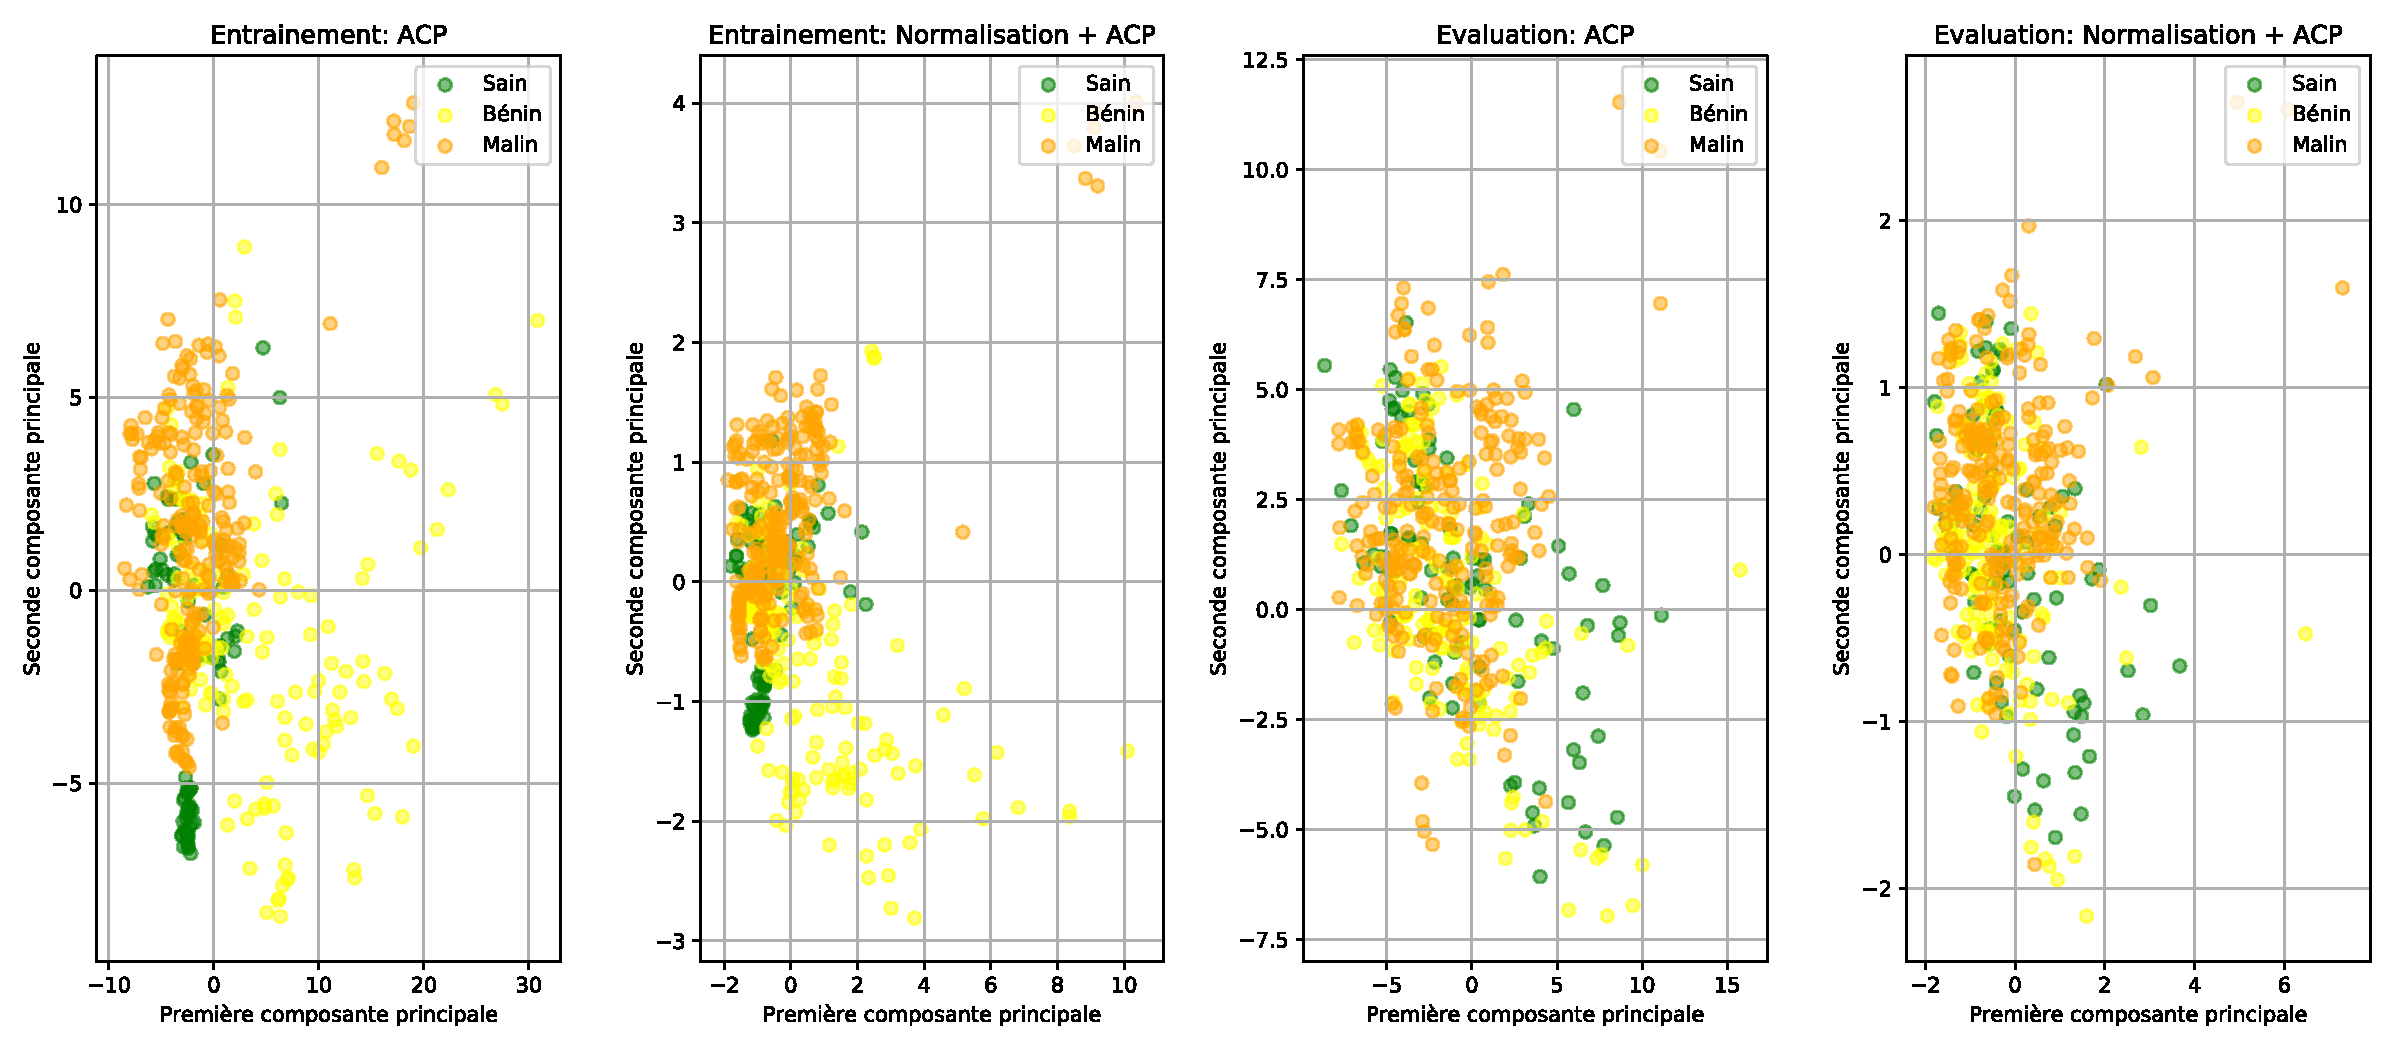
\includegraphics[width=\linewidth]{contents/chapter_4/resources/visualisation_scaling_PCA.pdf}
    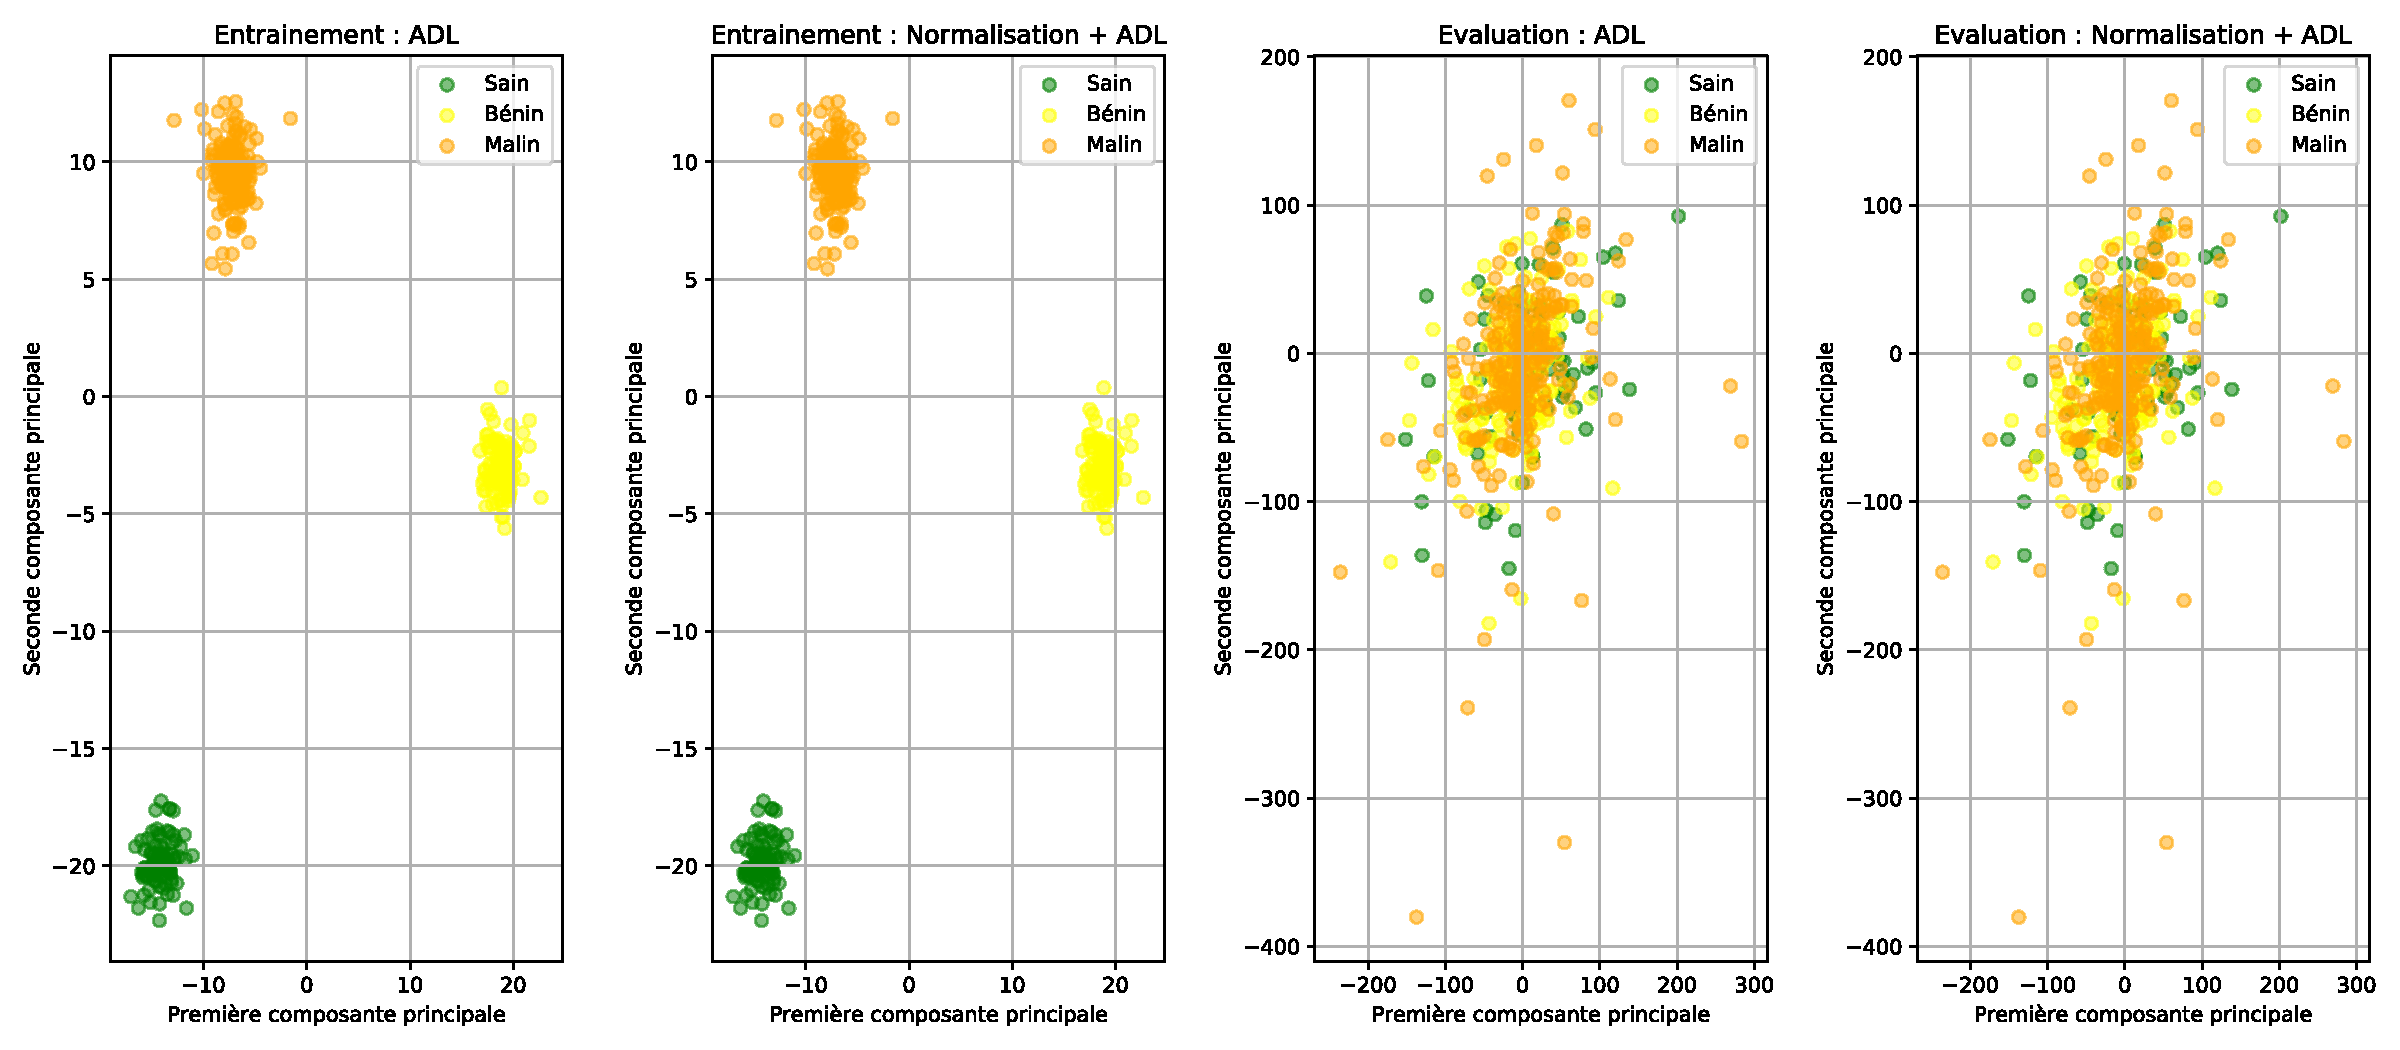
\includegraphics[width=\linewidth]{contents/chapter_4/resources/visualisation_scaling_LDA.pdf}
    \caption{Visualisation de l'influence de la réduction des dimensions appliquée au deux premières composantes principales, sur un échantillon constitué arbitrairement de 500 éléments de nos données. En haut, technique de réduction basée sur le \gls{pca} ; En bas, technique de réduction basée sur le \gls{lda}. A gauche, un processus procédant à la réduction puis à la normalisation ; A droite, un processus procédant à la normalisation puis à la réduction.}
    \label{fig:visualisation_scaling_reduction}
\end{figure}\par

\clearpage

\section{Résultats}
Les premières expérimentations menées sur les techniques d'extraction de caractéristiques associés aux techniques de normalisation nous permettent d'isoler celles d'entre elles jugées comme les plus pertinentes. Dans un premier temps du point de vue des techniques d'extraction spatial, nous obtenons un score maximal pour les caractéristiques proposé par Haralick non moyennés de 0,64 associés un écart-type de 0,07. Ce score est maximisé par l'utilisation par l'utilisation conjointe d'un modèle \gls{svm} avec noyau RBF et d'une normalisation par Minimum/Maximum. Dans un second temps du point de vue des techniques fréquentielles, le score de classification à trois classes est rendu maximal par l'utilisation de l'extraction en ondelettes de Daubechies par l'obtention d'un score de 0,67 associé à un écart type de 0,06. Ce score est maximisé par l'utilisation par l'utilisation conjointe d'un modèle \gls{svm} avec noyau linéaire ou RBF et d'une normalisation par Minimum/Maximum ou Standard. Enfin, par l'utilisation de diverses architectures de \gls{cnn}, nous parvenons à obtenir un score de de 0,77 associé à un écart type de 0,04 sur l'architecture ResNet-50 combinée à une couche de pooling moyen. Ce score est maximisé à l'aide d'un modèle \gls{svm} avec noyau linéaire et de la normalisation Minimum/Maximum. L'ensemble des résultats liées à cette première expérience sont visibles sur la \Cref{fig:results_image_classification} et sont détaillés en annexe.\par

\begin{figure}[H]
    \centering
    
    \begin{subfigure}{\textwidth}
      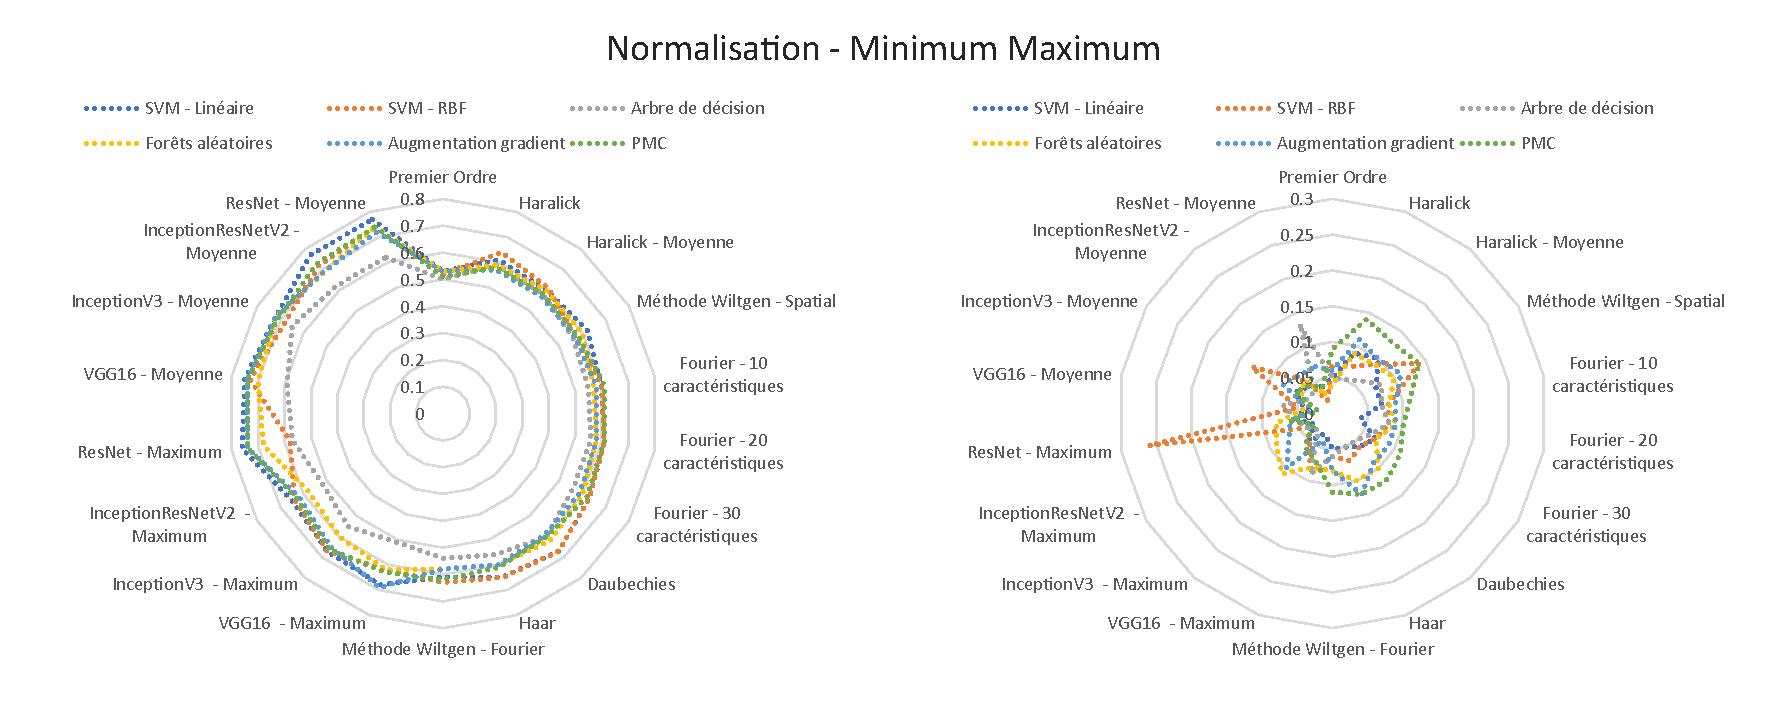
\includegraphics[width=\textwidth]{contents/chapter_4/resources/results_image_classification_mms.pdf}
    \end{subfigure}
    
    \begin{subfigure}{\textwidth}
      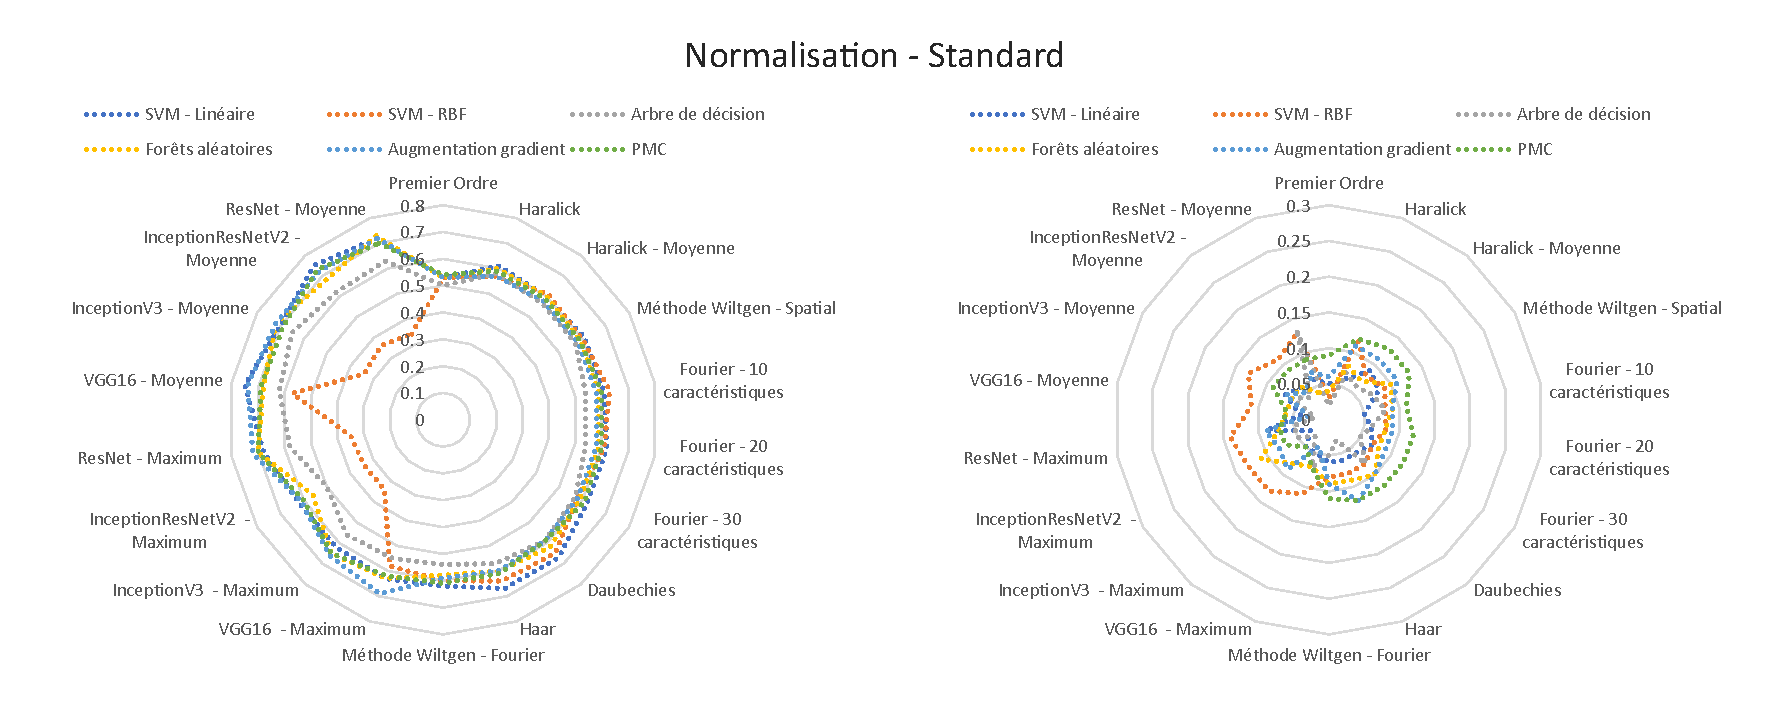
\includegraphics[width=\textwidth]{contents/chapter_4/resources/results_image_classification_ss.pdf}
    \end{subfigure}
    
    \caption{Résultats issues de la classification par les diverses techniques d'extraction et, par les modèles de classification mentionnés en couleur. En haut, les résultats provenant de la normalisation par Minimum/Maximum ; En bas, les résultats provenant de la normalisation par score Standard. A gauche, la représentation basée sur les valeurs moyennes ; A droite, la représentation tenant compte de l'écart-type.}
    \label{fig:results_image_classification}
\end{figure}\par

Le second volet de ces expérimentations vise à mesurer l'impact de la réduction d'informations des techniques d'apprentissage par transfert. En effet, la grande quantité d'information issue de ces techniques peut provoquer une dégradation des performances de classification, et nous souhaitons vérifier cette hypothèse par cette expérience. Seules les architectures précédemment évoquées couplées à une couche de global pooling moyen seront évaluées, leurs performances ayant été significativement supérieures à celle ayant un global pooling maximum. D'une part, la technique de réduction basée sur l'\gls{pca} a permis d'obtenir un score maximal de 0,76 et un écart-type plus restreint de 0,03 lorsque la variance cumulée est de 99\%. Ce score est obtenu avec l'utilisation de l'architecture ResNet-50 avec un pooling moyen, d'une normalisation par Minimum/Maximum et d'un modèle \gls{svm} linéaire. D'autre part, la technique de réduction basée sur le \gls{lda} nous permet de maximiser le score à une valeur de de 0,73 et un écart-type de 0,05 à partir d'une valeur de variance cumulée de 95\%. Ces valeurs sont obtenues par l'utilisation de l'architecture VGG-16 avec un pooling moyen, d'une normalisation Standard et d'un modèle \gls{svm} linéaire. L'ensemble des résultats de ce volet de l'expérience ont été reportés sur la \Cref{fig:results_image_classification_reduction}.\par

\begin{figure}[H]
    \centering
    
    \begin{subfigure}{\textwidth}
      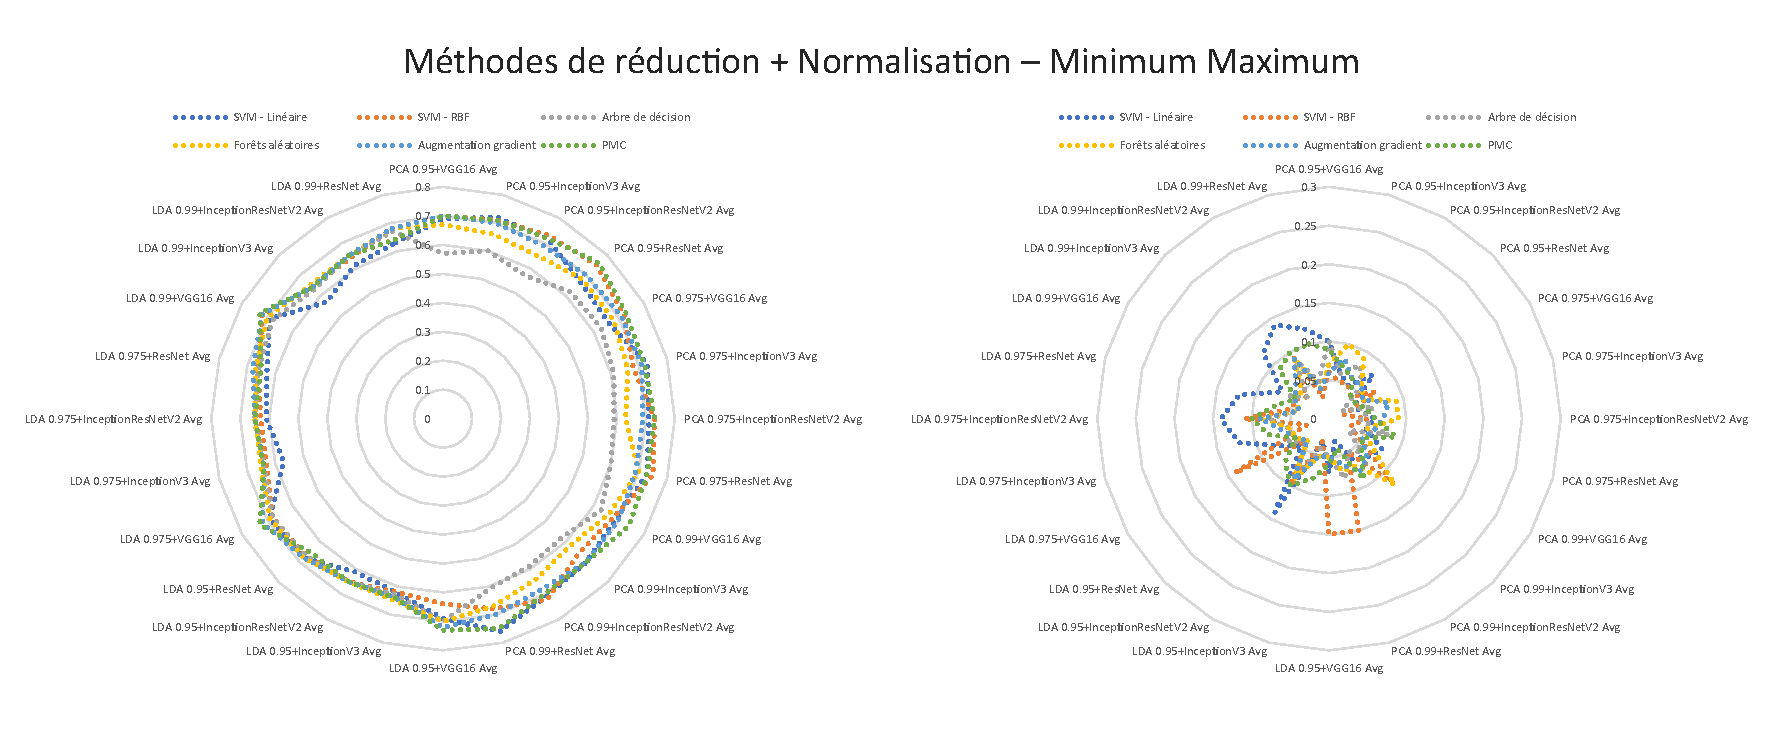
\includegraphics[width=\textwidth]{contents/chapter_4/resources/results_image_classification_reduction_mms.pdf}
    \end{subfigure}
    
    \begin{subfigure}{\textwidth}
      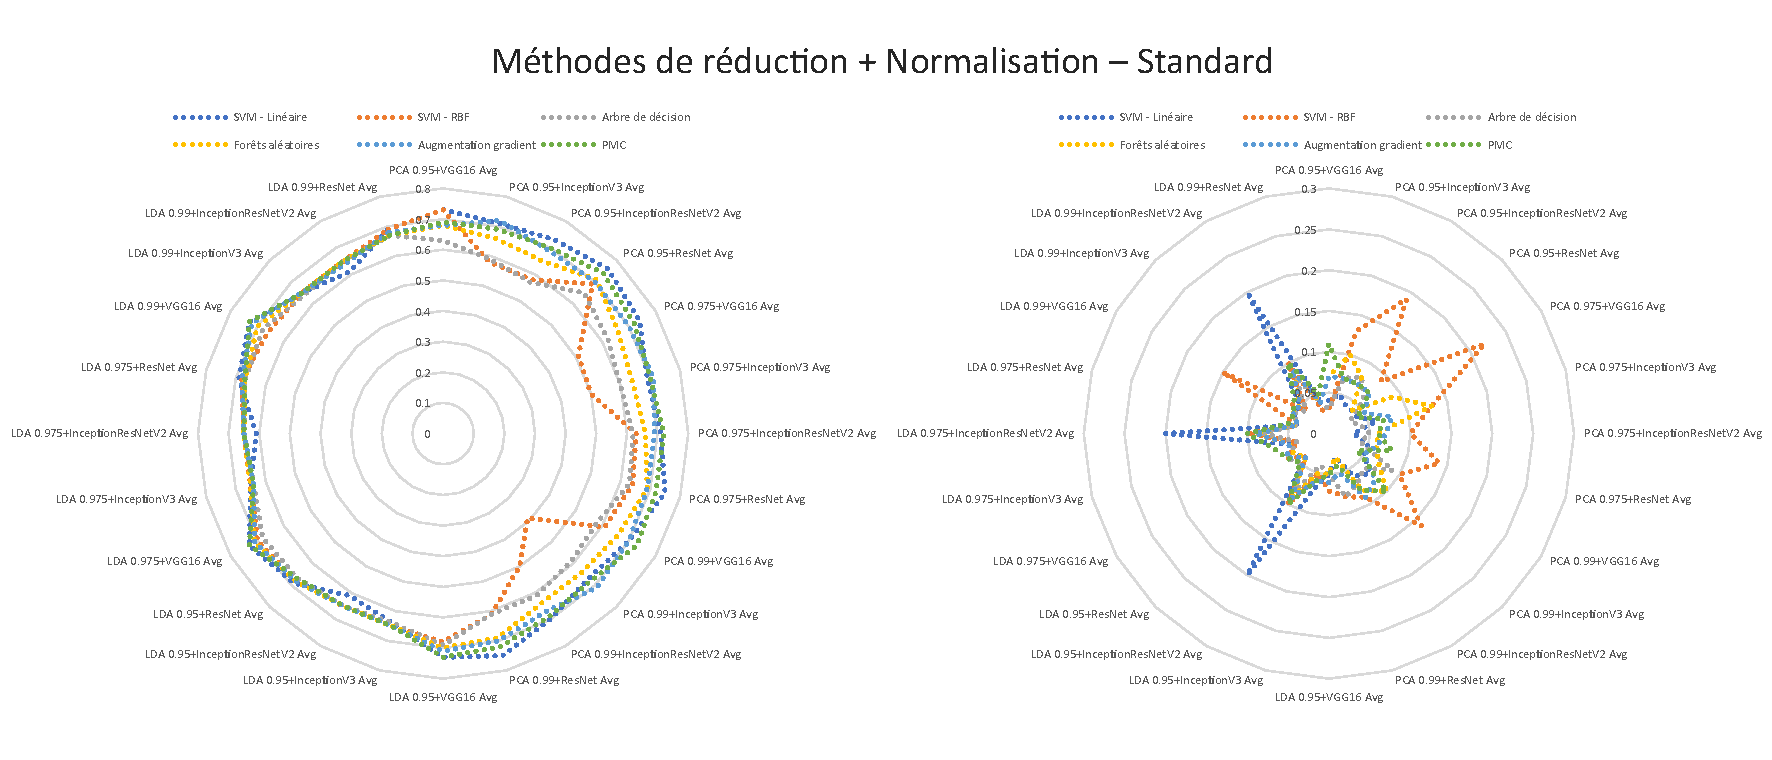
\includegraphics[width=\textwidth]{contents/chapter_4/resources/results_image_classification_reduction_ss.pdf}
    \end{subfigure}
    
    \caption{Résultats issues de la classification par l'utilisation de techniques de réduction combinés aux techniques d'extraction par transfert et, par les modèles de classification mentionnés en couleur. Les tracés de couleurs représentent les divers modèles évalués au cours de l'expérience. En haut, les résultats provenant de la normalisation par Minimum/Maximum ; En bas, les résultats provenant de la normalisation par score Standard. A gauche, la représentation basée sur les valeurs moyennes ; A droite, la représentation tenant compte de l'écart-type.}
    \label{fig:results_image_classification_reduction}
\end{figure}\par

La dernière partie de notre expérimentation vise à étudier l'impact de l'équilibrage des données sur la qualité des résultats de classification. Pour cela, les méthodes les plus performantes précédemment évoquées sont employées à cet usage. Ainsi, sur l'ensemble des méthodes évaluées la méthode par transfert, qui pour rappel emploie une architecture ResNet-50 avec un global pooling moyen et une normalisation Minimum/Maximum associée à un modèle \gls{svm} linéaire, atteint un score à trois classes de 0,77 et un écart type de 0,04. Ce score est obtenu avec l'utilisation d'une pondération dans le but de compenser le déséquilibre de données.\par

\begin{table}[H]
    \begin{tabular}{lllllll}
        \toprule
                    & Aucune    & Pond.             & Sur-éch. & Sous-éch. & SMOTE+ENN & SMOTE+Tomek\\ \hline
        Spatial     & 0.55±0.15 & 0.61±0.09         & 0.54±0.15& 0.58±0.11 & 0.60±0.09 & 0.56±0.16  \\
        Fréquentiel & 0.59±0.13 & 0.67±0.06         & 0.55±0.21& 0.58±0.17 & 0.61±0.12 & 0.64±0.10  \\
        \rowcolor[HTML]{E7E6E6}
        Transfert   & 0.71±0.08 & \textbf{0.77±0.04}& 0.74±0.07& 0.72±0.05 & 0.74±0.05 & 0.74±0.05  \\
        Réduction   & 0.71±0.09 & 0.76±0.03         & 0.74±0.06& 0.73±0.04 & 0.73±0.04 & 0.73±0.06  \\
        \bottomrule
    \end{tabular}
    \caption{Résultats à trois classes issus de l'expérience mêlant les méthodes les plus performantes associée aux méthodes de balancement de données évoquées.}
    \label{tab:results_balancement_multi}
\end{table}\par

Du point de vue de la séparation des tissus malins du reste des tissus, la méthode basée sur l'apprentissage par transfert par l'utilisation d'une architecture ResNet-50 avec un global pooling moyen et une normalisation Minimum/Maximum associée à un modèle \gls{svm} linéaire, reste la plus performante avec un score de 0,82 et un très faible écart-type de 0,01.\par

\begin{table}[H]
    \begin{tabular}{lllllll}
        \toprule
                    & Aucune    & Pond.             & Sur-éch.  & Sous-éch. & SMOTE+ENN & SMOTE+Tomek\\ \hline
        Spatial     & 0.65±0.11 & 0.63±0.07         & 0.64±0.10 & 0.64±0.08 & 0.63±0.09 & 0.59±0.27  \\
        Fréquentiel & 0.70±0.09 & 0.68±0.03         & 0.66±0.09 & 0.66±0.09 & 0.61±0.22 & 0.66±0.09  \\
        \rowcolor[HTML]{E7E6E6} 
        Transfert   & 0.81±0.04 & \textbf{0.82±0.02}& 0.81±0.03 & 0.79±0.01 & 0.80±0.02 & 0.82±0.03  \\
        Réduction   & 0.81±0.03 & 0.81±0.01         & 0.81±0.03 & 0.79±0.03 & 0.80±0.01 & 0.81±0.03  \\
        \bottomrule 
    \end{tabular}
    \caption{Résultats de la détection de tissus malin issus de l'expérience mêlant les méthodes les plus performantes associée aux méthodes de balancement de données évoquées.}
    \label{tab:results_balancement_malignant}
\end{table}\par

Enfin, une les courbes \gls{roc} nous permettent d'appréhender les performances de prédiction de ce système. Ainsi, les performances propre à l'ensemble de la base d'images annotés sont homogènes par cette technique avec des scores \gls{auc} compris entre 0,87 et 0,90. Néanmoins, une analyse \gls{roc} des lésions \gls{lm} et \gls{lmm} permet de mettre en avant des performances moins homogènes entre les diverses classes pouvant montrer des difficultés de cette techniques à séparer les tissus de ces lésions, les score \gls{auc} variant entre 0,79 et 0,92. Ces éléments sont visibles sur la \Cref{fig:results_image_classification_roc}.\par

\begin{figure}[H]
    \centering
    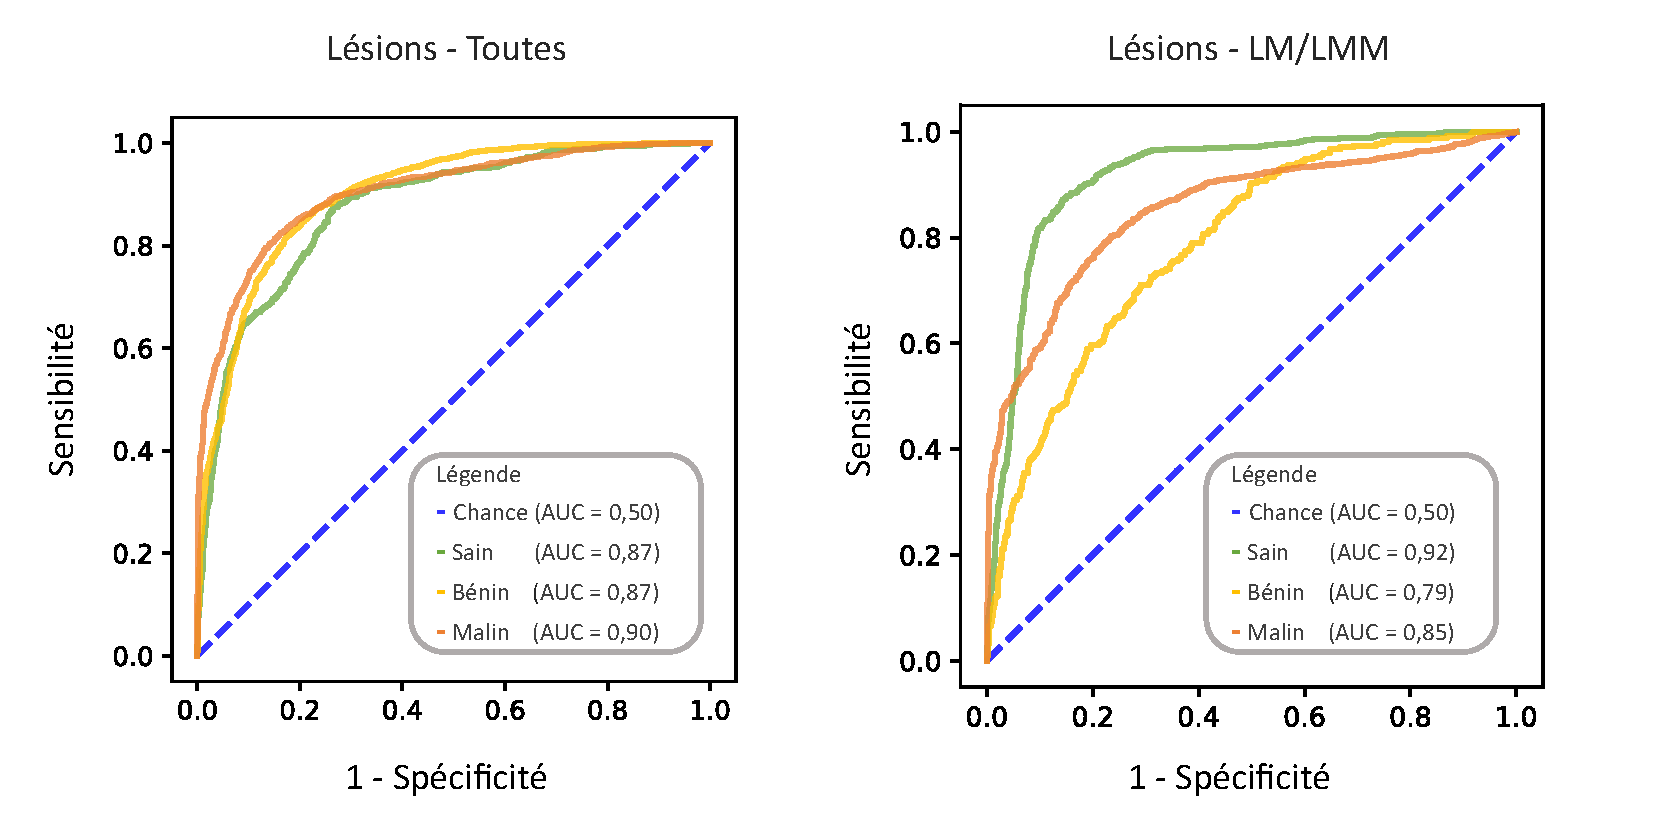
\includegraphics[width=\textwidth]{contents/chapter_4/resources/results_image_classification_roc.pdf}
    \caption{Courbes \gls{roc} et scores \gls{auc} associés aux courbes. A gauche, courbes associées à l'ensemble des lésions d'étude ; A droite, courbes associées aux seules cas pathologiques de \gls{lm}/\gls{lmm}.}
    \label{fig:results_image_classification_roc}
\end{figure}\par

\section{Discussion}
A la suite des précédents résultats, il nous est possible dans un premier temps de formuler divers constats pour donner suite à la mise en pratique des diverses méthodes d'extraction de caractéristiques. La première d'entre elle sur les caractéristiques spatiales, met en avant l'utilité de la méthode d'Haralick sur ces données de \gls{rcm}, mais pour lesquelles l'ajout de mesures de premier ordre ne semble pas ou peu impacter le résultat. La seconde d'entre elle concerne les caractéristiques fréquentielles, et sur l'utilité de l'extraction en ondelettes comparée aux caractéristiques extraites à l'aide de l'espace de Fourier sur ces mêmes données. Nous avons également montré une faible influence de l'ondelette mère, bien que celle de Daubechies soit pertinente sur nos données. Enfin, la proposition de méthode employant des architectures de \gls{cnn} pour l'extraction de caractéristiques a été la plus pertinente d'entre toute, notamment par l'utilisation de couche de global pooling moyen. Sur l'ensemble des architectures évalués, ResNet-50 semble être celle allant dans le sens de notre problématique que nous développerons par la suite.\par

En ce qui concerne les modèles de classification employés, nous pouvons constater que le modèle \gls{svm} à noyau linéaire a été le plus pertinent dans la plupart des expériences menées lors de ce chapitre. Le modèle \gls{svm} à noyau RBF a été essentiellement pertinent à l'aide d'une normalisation par Minimum/Maximum, sa performance et stabilité chutant de manière drastique lorsque les caractéristiques sont nombreuses, comme avec les méthodes par transfert de connaissance. Du côté des méthodes basées sur les arbres de décisions, ces techniques ont été globalement peu influencées par les méthodes de normalisation. Comme attendu, les \gls{cart} ont été performant dans la plupart des situations, exceptée celles par transfert de connaissances dans lesquelles le nombre de caractéristiques est trop important. A cette fin, les techniques de \gls{rf} et \gls{gb} ont été particulièrement adaptées, les \gls{gb} étant légèrement moins stables que les \gls{rf}. Pour finir cette analyse des modèles, l'utilisation de \gls{mlp} dans le but d'observer l'effet de la non-linéarité semble ne pas avoir aidé à améliorer la classification.\par

Afin de compenser le nombre élevé des caractéristiques extraites par les \gls{cnn}, des techniques de réduction ont été mise en œuvre afin de pallier ce problème. Leur utilisation aura réduit les performances globales du système mais également la stabilité en augmentant l'écart-type sensiblement. Néanmoins, des performances non négligeables ont été obtenues dans une configuration utilisant ResNet-50 et l'\gls{pca} avec une variance expliquée de 99\%, avec moins d'un quart des caractéristiques. La variance expliquée obtenue par \gls{pca} est visible sur la \Cref{fig:results_image_classification_pca_variance}.\par

\begin{figure}[H]
    \centering
    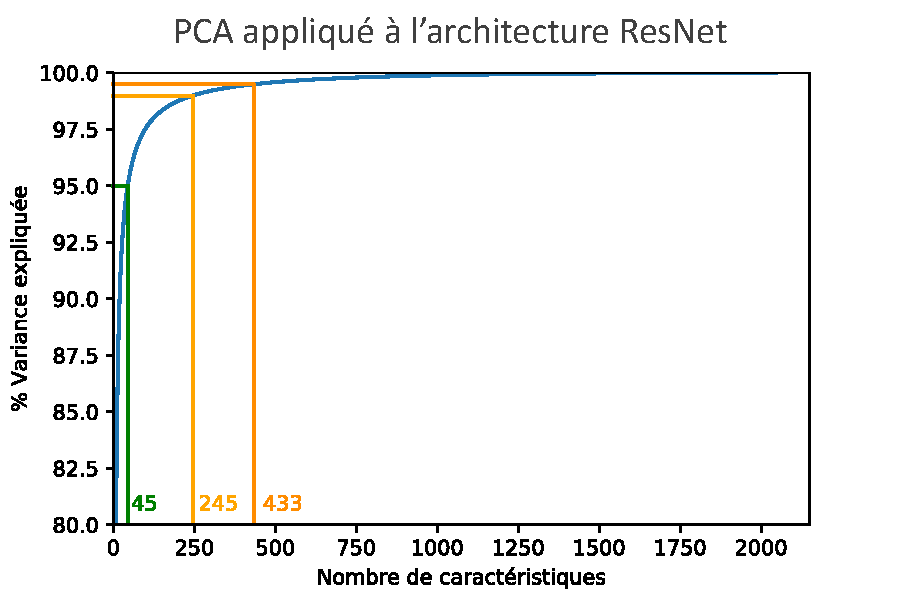
\includegraphics[width=0.6\textwidth]{contents/chapter_4/resources/results_image_classification_pca_variance.pdf}
    \caption{Analyse de la variance expliquée cumulée par l'application de l'\gls{pca}. Une variance cumulée de 95\% peux être obtenue à l'aide de 45 caractéristiques tandis qu'une variance cumulée de 99,5\% peux être obtenue à l'aide de 433 caractéristiques.}
    \label{fig:results_image_classification_pca_variance}
\end{figure}\par

La dernière méthode mise en œuvre pour optimiser les performances de classification des images concerne le balancement des annotations. Nous avons initialement favorisé la pondération, proposant une correction des non-balancement à moindre frais, mais sans certitude sur sa pertinence. Sur les diverses méthodes évaluées lors de ces expériences, la pondération à permis l'obtention des meilleurs résultats avec un coup de mise en place faible sur nos données.\par

En conclusion, ce premier chapitre expérimental aura permis de mettre au point un processus permettant de traiter les données \gls{rcm}. Nous avons pu ainsi accomplir une classification avec un \fscore{} de 0,77 et un écart-type de 0,04 pour 3 classes et 0,82 et un écart-type de 0,02 pour la classification d'éléments malins. De plus ce processus aura permis l'obtention d'une \gls{auc} de 0,90 sur l'ensemble des images malignes et de 0,85 sur les images malignes d'origine \gls{lm}/\gls{lmm}.\par

Néanmoins, notre proposition de technique ne prend en compte que la caractérisation des tissus des images. Une amélioration possible de ces expériences pourrait prendre en compte l'intersection d'évènements tels que la présence de tissus caractéristiques et la présence de follicules pileux conjointement.\par